\documentclass[12pt,oneside]{report}

%% ---------------------------------------------------------------
%%  PACKAGES
%% ---------------------------------------------------------------
\usepackage[margin=1in]{geometry}
\usepackage{times}
\usepackage{setspace}
\usepackage{graphicx}
\usepackage{float}
\usepackage{booktabs}
\usepackage{longtable}
\usepackage{array}
\usepackage{multirow}
\usepackage{amsmath}
\usepackage{amssymb}
\usepackage{url}
\usepackage{hyperref}
\usepackage{cite}
\usepackage{fancyhdr}
\usepackage{titlesec}
\usepackage{tocloft}
\usepackage{caption}
\usepackage{subcaption}
\usepackage{xcolor}
\usepackage{enumitem}
\usepackage{tabularx}
\usepackage{rotating}
\usepackage{pdfpages}
\usepackage{etoolbox}
\usepackage{tikz}
\usepackage{pgfplots}
\pgfplotsset{compat=1.17}
\usetikzlibrary{shapes,arrows,positioning,calc,fit,backgrounds}
\hyphenpenalty=10000
\exhyphenpenalty=10000
\sloppy

%% ---------------------------------------------------------------
%%  FORMAT SETTINGS
%% ---------------------------------------------------------------
\doublespacing
\setlength{\parindent}{0.5in}
\setlength{\parskip}{0pt}

% Chapter title formatting - ALL CAPS, centered
\newcommand{\chapterlabel}{CHAPTER}
\titleformat{\chapter}[display]
  {\normalfont\large\bfseries\centering}
  {\chapterlabel\ \thechapter}
  {0pt}
  {\large\MakeUppercase}
\titlespacing{\chapter}{0pt}{0pt}{2\baselineskip}

% Appendix format: APPENDIX A, APPENDIX B, etc.

% Section formatting
\titleformat{\section}{\normalfont\normalsize\bfseries}{\thesection}{1em}{}
\titleformat{\subsection}{\normalfont\normalsize\bfseries}{\thesubsection}{1em}{}
\titleformat{\subsubsection}{\normalfont\normalsize\itshape}{\thesubsubsection}{1em}{}

% Header/footer
\pagestyle{fancy}
\fancyhf{}
\fancyhead[R]{\thepage}
\renewcommand{\headrulewidth}{0pt}

% Caption format
\captionsetup[figure]{labelfont=bf,position=below}
\captionsetup[table]{labelfont=bf,position=above}

% Hyperlink colors
\hypersetup{colorlinks=true,linkcolor=black,citecolor=black,urlcolor=black}

%% ---------------------------------------------------------------
%%  DOCUMENT
%% ---------------------------------------------------------------
\begin{document}
\graphicspath{{./}{poster_figures/}}
\pagenumbering{gobble}

%% ==============================================================
%%  TITLE PAGE
%% ==============================================================
\begin{titlepage}
\begin{center}
\vspace*{0.5in}

{\large CARNEGIE MELLON UNIVERSITY}

\vspace{0.3in}

{\large CARNEGIE INSTITUTE OF TECHNOLOGY}

\vspace{0.5in}

\rule{\textwidth}{1pt}

\vspace{0.3in}

{\large\bfseries AI-Augmented Compliance Auditing for Cloud Systems:\\[6pt]
A Hybrid ML--LLM Approach}

\vspace{0.3in}

\rule{\textwidth}{1pt}

\vspace{0.5in}

{\large THESIS}

\vspace{0.3in}

{\large SUBMITTED IN PARTIAL FULFILLMENT OF THE REQUIREMENTS\\
FOR THE DEGREE OF}

\vspace{0.3in}

{\large\bfseries Master of Science}

\vspace{0.3in}

{\large IN}

\vspace{0.3in}

{\large\bfseries Information Technology}

\vspace{0.5in}

{\large BY}

\vspace{0.3in}

{\large\bfseries Moise Iradukunda Ingabire}

\vspace{0.5in}

\begin{tabular}{ll}
\textbf{Thesis Advisor:} & Professor Jema David Ndibwile \\[6pt]
\textbf{Department:} & Engineering and Technology \\[6pt]
\textbf{Institution:} & Carnegie Mellon University Africa \\[6pt]
\textbf{Location:} & Kigali, Rwanda \\[6pt]
\textbf{Date:} & May 2026
\end{tabular}

\vfill

{\large Carnegie Mellon University Africa, Kigali, Rwanda}

\vspace{0.2in}

{\small Copyright \textcopyright\ 2026 Moise Iradukunda Ingabire. All rights reserved.}

\end{center}
\end{titlepage}

%% ==============================================================
%%  COMMITTEE PAGE
%% ==============================================================
\newpage
\thispagestyle{empty}
\begin{center}
\vspace*{0.8in}

{\large\bfseries THESIS}

\vspace{0.3in}

{\large SUBMITTED IN PARTIAL FULFILLMENT OF THE REQUIREMENTS}

\vspace{0.2in}

{\large FOR THE DEGREE OF \textbf{Master of Science}}

\vspace{0.5in}

\begin{tabular}{@{}p{0.35\textwidth}p{0.60\textwidth}@{}}
\textbf{TITLE:} & AI-Augmented Compliance Auditing for Cloud Systems: A Hybrid ML--LLM Approach \\[18pt]
\textbf{PRESENTED BY:} & Moise Iradukunda Ingabire \\[18pt]
\textbf{ACCEPTED BY THE} & \\
\textbf{DEPARTMENT OF:} & Engineering and Technology \\[18pt]
\textbf{THESIS ADVISOR:} & Professor Jema David Ndibwile \\[18pt]
\textbf{ACADEMIC ADVISOR:} & Emmanuel Ndashimye \\
                            & Assistant Teaching Professor \\[18pt]
\textbf{DEPARTMENT HEAD:} & George Okeyo Onyango \\
\end{tabular}

\end{center}

%% ==============================================================
%%  DEDICATION
%% ==============================================================
\newpage
\thispagestyle{empty}
\vspace*{2in}
\begin{center}
\textit{To the people of Rwanda,\\
whose digital future this work seeks to secure.\\[12pt]
And to my family,\\
whose unwavering support made this journey possible.}
\end{center}

%% ==============================================================
%%  ACKNOWLEDGMENTS
%% ==============================================================
\newpage
\pagenumbering{roman}
\setcounter{page}{4}
\chapter*{ACKNOWLEDGMENTS}
\addcontentsline{toc}{chapter}{Acknowledgments}

I am deeply grateful to my thesis advisor, Professor Jema David Ndibwile, whose mentorship, critical insight, and unwavering support shaped every dimension of this research. His expertise in cybersecurity and his commitment to African technological advancement provided the intellectual scaffolding that grounded this work in both technical rigor and real-world relevance.

I wish to acknowledge Carnegie Mellon University Africa for providing an exceptional academic environment at the intersection of global excellence and African context. The institution's mission to develop technically and professionally skilled graduates who will transform the African continent has been both a challenge and an inspiration throughout this program.

My gratitude extends to the Rwanda National Cyber Security Authority (NCSA) for establishing the Minimum Cybersecurity Standards framework that motivated this research. By codifying 169 controls across six families, the NCSA has created the precise kind of structured regulatory artifact that AI-augmented auditing can make operationally accessible to institutions that lack large compliance teams.

I acknowledge the open-source community whose tools—XGBoost, scikit-learn, LangChain, FastAPI, Kubernetes, and many others—made rapid prototyping and rigorous evaluation possible. I am likewise indebted to the researchers behind public datasets (SecRepo, LANL, LogHub, NSL-KDD) that enabled systematic experimentation.

To my colleagues at CMU Africa: the late-night study sessions, the critical debates in seminar rooms, and the shared burden of ambition have been invaluable. Special thanks are due to those who provided informal peer review on early drafts of this thesis.

Finally, I acknowledge the use of AI language models (GPT-4o, GPT-4o-mini, and LLaMA 3) during this project—both as evaluated components of the compliance-auditing system under experimental study and to assist with manuscript drafting. All AI-assisted content has been reviewed, edited, and verified by the author, who takes full responsibility for every claim in this document.

%% ==============================================================
%%  ABSTRACT
%% ==============================================================
\newpage
\chapter*{ABSTRACT}
\addcontentsline{toc}{chapter}{Abstract}

Automated compliance auditing in Africa remains severely under-resourced: most institutions rely on manual checklists executed infrequently by staff with limited forensic depth, leaving critical security gaps undetected between audit cycles. This thesis presents an AI-augmented compliance auditor that combines multi-label machine learning with Large Language Model (LLM) reasoning, validated on Rwanda's National Cyber Security Authority (NCSA) Minimum Cybersecurity Standards—a 169-control framework aligned with NIST SP 800-53 Rev.\ 5.

The system implements 143 of 169 NCSA controls (85\% coverage) through 60 specialized evidence parsers that execute native operating-system audit commands and interpret their output against control-specific compliance criteria. A seven-engine microservices architecture handles the complete audit pipeline: log ingestion, document processing, LLM-augmented analysis via the Model Context Protocol (MCP), decision orchestration, web-based reporting, and authentication. The system deploys on Kubernetes with 2.0 CPU cores and 2.66\,GB RAM at approximately \$50/month.

Multi-label XGBoost (30 features: 5 numeric + 25 TF-IDF) achieves 99.88\% F1 on real logs after 5\% target-domain fine-tuning, but collapses to 7.98\% zero-shot F1 on unseen log formats—exposing the fundamental generalization gap of vocabulary-based models. GPT-4o-mini achieves 93.5\% zero-shot accuracy across four log types ($n$\,=\,200): SSH (84\%), macOS System (92\%), HTTP/API (98\%), and Windows Events (100\%), while Llama-3.2-3B on CPU-only hardware achieves 84.0\%, demonstrating viable on-premise LLM deployment for African SMEs. A vocabulary-coverage gating router ($\nu \geq \theta = 0.20$) achieves 94.5\% accuracy at \$0.149/10K logs—a +5.4 percentage-point improvement over static routing.

Adversarial validation reveals effectiveness gaps invisible to presence-based auditing: SI-3 (Malware Protection) achieves only 20\% fileless-shell detection; SI-10 (Input Validation) remains non-compliant at 32\% XSS bypass despite WAF deployment. A theoretical effectiveness model $C(k) = \alpha D_k + \beta V_k + \gamma R_k$ formalizes compliance as a continuous, measurable function replacing binary presence checking.

Live deployment on a production macOS system achieved 75\% compliance in a 0.77-second automated audit (Audit ID: AUDIT-20260320-205239). This research provides a replicable blueprint for AI-augmented compliance auditing across African nations pursuing cybersecurity maturity under the Malabo Convention.

\textbf{Keywords:} compliance auditing, machine learning, large language models, cybersecurity, NCSA, NIST SP 800-53, Rwanda, XGBoost, multi-label classification, hybrid AI

%% ==============================================================
%%  TABLE OF CONTENTS
%% ==============================================================
\newpage
\tableofcontents

%% ==============================================================
%%  LIST OF FIGURES
%% ==============================================================
\newpage
\listoffigures
\addcontentsline{toc}{chapter}{List of Figures}

%% ==============================================================
%%  LIST OF TABLES
%% ==============================================================
\newpage
\listoftables
\addcontentsline{toc}{chapter}{List of Tables}

%% ==============================================================
%%  LIST OF ABBREVIATIONS
%% ==============================================================
\newpage
\chapter*{LIST OF ABBREVIATIONS}
\addcontentsline{toc}{chapter}{List of Abbreviations}

\setstretch{1.0}
\begin{longtable}{|p{1.5in}|p{4.5in}|}
\hline
\textbf{Abbreviation} & \textbf{Full Form} \\
\hline
\endhead
AC  & Access Control \\
AI  & Artificial Intelligence \\
API & Application Programming Interface \\
AU  & Audit and Accountability \\
AV  & Antivirus \\
BERT & Bidirectional Encoder Representations from Transformers \\
CIS & Center for Internet Security \\
CM  & Configuration Management \\
CPU & Central Processing Unit \\
CV  & Cross-Validation \\
DL  & Deep Learning \\
EDR & Endpoint Detection and Response \\
F1  & F1-Score (harmonic mean of precision and recall) \\
GPT & Generative Pre-trained Transformer \\
IA  & Identification and Authentication \\
ISO & International Organization for Standardization \\
ITU & International Telecommunication Union \\
JWT & JSON Web Token \\
LLM & Large Language Model \\
LSTM & Long Short-Term Memory \\
MCP & Model Context Protocol \\
ML  & Machine Learning \\
NCSA & National Cyber Security Authority (Rwanda) \\
NGINX & Engine X (open-source web server / reverse proxy) \\
NIST & National Institute of Standards and Technology \\
NLP & Natural Language Processing \\
RBAC & Role-Based Access Control \\
RAM & Random Access Memory \\
SC  & System and Communications Protection \\
SHAP & SHapley Additive exPlanations \\
SI  & System and Information Integrity \\
SIEM & Security Information and Event Management \\
SME & Small and Medium Enterprise \\
SOC & Security Operations Center \\
TF-IDF & Term Frequency–Inverse Document Frequency \\
WAF & Web Application Firewall \\
XGBoost & Extreme Gradient Boosting \\
XSS & Cross-Site Scripting \\
\hline
\end{longtable}

%% ==============================================================
%%  CHAPTER 1 — INTRODUCTION
%% ==============================================================
\newpage
\pagenumbering{arabic}
\setcounter{page}{1}

\chapter{INTRODUCTION}

\section{Background and Motivation}

\subsection{The Problem Behind the Problem}

Consider a compliance officer at a Rwandan public institution in the months following the enactment of the National Cyber Security Authority (NCSA) Minimum Cybersecurity Standards in 2023 \cite{ncsa2023}. Her mandate is clear: 169 security controls must be assessed, evidenced, and reported for every system under her institution's management. The controls are well-defined. The deadline is fixed. The regulator is watching.

What she cannot do—with a team of four, a spreadsheet, and manual audit procedures—is perform this assessment continuously, comprehensively, or with any depth beyond the surface question of whether a control is technically present. She can verify that an antivirus product is installed; she cannot test whether it detects fileless shell attacks. She can confirm that a Web Application Firewall is deployed; she cannot determine whether it blocks cross-site scripting. She can check that audit logging is configured; she cannot parse 60 days of authentication records against 143 simultaneous compliance criteria before the working day ends. The standard is rigorous. The means to meet it continuously are not.

This thesis was motivated by that gap—not as an abstract research problem, but as a lived operational reality in the institutions that Rwanda's digital transformation depends upon. The research question is simple to state and difficult to solve: can AI-augmented automation transform compliance auditing from an infrequent, expensive, shallow exercise into a continuous, affordable, technically deep capability? The answer this thesis provides is: yes—and the system built to prove it audits 143 NCSA controls in 0.77 seconds, at \$50 per month, on hardware that any institution can afford.

\subsection{Rwanda's Digital Ambition and the Security Imperative}

Rwanda's transformation into a continental technology hub is one of the most deliberate national development stories of the twenty-first century. Through Vision 2050 and the Smart Rwanda Master Plan, the government has systematically digitized government services, financial infrastructure, and healthcare systems at a pace that has few parallels in the developing world. By 2024, more than 90\% of public services were accessible digitally, mobile money transactions exceeded the GDP of several neighboring countries in monthly volume, and the Kigali Innovation City had attracted technology companies from across the globe.

This digital ambition carries a security obligation that scales directly with the ambition itself. Every digitized service is a potential attack surface. Every database of citizen records is a target. Every cloud-hosted government system that lacks continuous security monitoring represents a liability that undermines the very transformation it is meant to serve. Serianu's 2023 Africa Cyber Security Report documented that African nations collectively lost an estimated \$4 billion to cybercrime annually \cite{serianu_africa}, with public institutions disproportionately targeted due to their high-value data holdings and often-limited security budgets. Rwanda, precisely because it has digitized faster than most, faces this exposure more acutely than most.

The ITU's Global Cybersecurity Index 2024 \cite{itu_africa_cyber} placed Rwanda among the top five African nations on commitment measures—reflecting the quality of its regulatory architecture and legislative intent. What it could not measure, because no instrument exists for it at national scale, is the gap between regulatory intent and operational implementation across the hundreds of institutions subject to the NCSA framework \cite{ncsa2023}. That gap is this thesis's domain.

The African Union's Malabo Convention on Cyber Security and Personal Data Protection \cite{malabo2014} establishes a continental mandate for cybersecurity governance that Rwanda has been among the first to operationalize. As seventeen AU member states have now ratified the Convention \cite{au_cybersecurity_status}, the compliance frameworks they develop—Rwanda's NCSA MCS foremost among them—will define the technical baseline for digital security across the continent. Research that makes Rwanda's framework operationally enforceable therefore has implications far beyond Rwanda's borders.

\subsection{The Insufficiency of Existing Tools}

The global compliance automation market is not without products. Tools such as OpenSCAP \cite{openscap} and Wazuh \cite{wazuh_ref} have made genuine contributions to automated security assessment, providing script-based configuration checking and rule-based log alerting that reduce the manual burden for specific control domains. Cloud providers offer native compliance dashboards tied to their own service APIs. Commercial SIEM platforms such as Splunk and IBM QRadar provide log aggregation and correlation at scale.

None of these tools address the compliance challenge as it presents itself at a Rwandan public institution. They were designed for well-resourced IT departments in North American or European contexts, with dedicated compliance teams, extensive labeled training data from the specific log formats in use, and the budget to license commercial SIEM platforms at enterprise pricing. They do not implement the NCSA framework. They do not provide multi-label classification against national control families. They do not combine evidence collection, ML-based log analysis, LLM-augmented semantic reasoning, and structured regulatory reporting in a single deployable system that costs \$50 per month.

More fundamentally, existing tools do not challenge the binary assumption at the heart of compliance auditing: that a control is either present or absent, compliant or not, checked or unchecked. The Ponemon Institute's 2023 compliance cost benchmark \cite{ponemon_cost} documented that organizations spend an average of \$5.47 million annually on compliance activities, yet the primary output of this investment is a checklist—a binary verdict that says nothing about whether the controls on it actually work. This thesis's adversarial validation results, presented in Chapter 4, demonstrate concretely that this binary paradigm fails: an antivirus rated ``compliant'' under presence-based auditing may detect only 20\% of contemporary fileless attack techniques; a WAF rated ``compliant'' may allow 32\% of tested XSS payloads to bypass it. The compliance investment is real. The security assurance it purchases is not.

\subsection{Why This Research, Why Now, Why Here}

The timing of this research reflects a convergence of three developments that did not coexist until recently:

\textbf{Large Language Models with genuine zero-shot reasoning capability.} The arrival of GPT-4o, Llama 3, and Mistral as practical, affordable inference engines—including through locally deployable variants that eliminate API dependency—has made it possible for the first time to apply semantic understanding to compliance log analysis without requiring thousands of domain-specific labeled examples \cite{karlsen2024}. An LLM that understands the intent of NCSA IA-2 can assess an authentication log it has never seen before. This capability did not exist at the scale and cost point necessary for institutional deployment three years ago.

\textbf{The Model Context Protocol as an LLM-to-tool integration standard.} Anthropic's introduction of the Model Context Protocol (MCP) in late 2024 \cite{mcp_anthropic} provided the architectural primitive needed to connect LLM reasoning to structured evidence collection pipelines. Without MCP—or an equivalent standard—LLM-based compliance analysis would be limited to prompting models with raw log text and hoping for consistent output. MCP enables the system designed in this thesis to expose typed tools (evidence collectors, control evaluators, finding recorders) to the LLM in a structured, auditable manner.

\textbf{Rwanda's NCSA framework as a well-defined, NIST-aligned target.} The 2023 Minimum Cybersecurity Standards \cite{ncsa2023} arrived with the specificity needed for AI implementation: 169 controls, organized into six families, with clearly stated assessment criteria aligned to NIST SP 800-53 Rev. 5 \cite{nist2020}. This level of specification is what makes machine implementation possible. A vague regulatory requirement cannot be programmed; a precisely defined control with documented evidence criteria can.

The author's position as a graduate student at Carnegie Mellon University Africa—trained in global AI research methods and embedded in the Rwandan institutional context—created a unique vantage point from which to see both the technical possibility and the institutional need simultaneously. This thesis is the product of that vantage point: a system built using world-class AI methods to solve a problem that is specific, urgent, and real in the institutions visible from the CMU Africa campus in Kigali.

\section{Problem Statement}

Three precisely defined problems motivate this research:

\textbf{Problem 1: The Automation Gap.} Existing compliance tools—OpenSCAP \cite{openscap}, Wazuh \cite{wazuh_ref}, and commercial SIEM platforms—do not address the multi-framework, multi-format log analysis required by comprehensive national standards such as the NCSA MCS. No existing system combines automated NCSA-specific evidence collection, multi-label ML classification, LLM semantic reasoning, and regulatory-grade report generation in a single deployable platform validated on an African national cybersecurity framework.

\textbf{Problem 2: The Generalization Gap.} Machine learning models trained on synthetic or benchmark log data exhibit catastrophic performance collapse when applied to novel real-world log formats. This generalization gap—not previously quantified in the compliance auditing literature for multi-label settings—undermines the practical deployability of pure ML approaches. A model that achieves 99.99\% F1 on its training distribution but 7.98\% on real deployment-environment logs is not a deployable compliance tool; it is a liability. Understanding this gap precisely—its magnitude, its mechanism, and its mitigation—is essential groundwork for any production AI compliance system.

\textbf{Problem 3: The Effectiveness Gap.} Compliance frameworks universally employ binary presence checking: a control is either implemented or absent. This paradigm fails to measure whether deployed controls actually protect what they are designed to protect. A firewall that blocks incorrect ports, an antivirus that misses fileless attacks, and an input validator with a 32\% XSS bypass rate are all rated ``compliant'' under binary auditing—yet they offer materially different protection than fully effective implementations. Without a quantitative effectiveness model validated through adversarial testing, compliance scores are claims about process, not evidence of security.

\section{Rwanda's Cybersecurity Landscape}

Rwanda's approach to national cybersecurity governance reflects both the sophistication of its regulatory ambitions and the operational challenges of translating policy into practice across a rapidly growing digital economy. The NCSA, established as an autonomous government agency, has taken deliberate steps to align Rwanda's security standards with global best practice. The 2023 Minimum Cybersecurity Standards \cite{ncsa2023} map directly to NIST SP 800-53 Rev.\ 5 \cite{nist2020}, selecting the six control families most relevant to the operational security of public institutions: Access Control (AC, 52 controls), Audit and Accountability (AU, 30 controls), Configuration Management (CM, 18 controls), Identification and Authentication (IA, 15 controls), System and Communications Protection (SC, 26 controls), and System and Information Integrity (SI, 2 controls)—totaling 169 mandatory controls.

The Rwanda National Cybersecurity Strategy 2024--2029 \cite{rwanda_strategy_2024} sets ambitious targets: automated compliance monitoring capabilities deployed across all regulated institutions, continuous security assessment replacing the current annual audit cycle, and Rwanda's compliance infrastructure serving as a model for the region. These are not merely aspirational targets; they represent the regulatory direction that institutions subject to NCSA oversight must plan for.

The threat context makes this urgency concrete. According to Serianu's 2023 report \cite{serianu_africa}, public sector institutions in Africa are the most frequently targeted category by cybercriminals, precisely because they hold high-value citizen data and often operate with limited security operations capabilities. Kenya's experience with cybercrime legislation \cite{kenya_cyber_law} and Nigeria's NITDA framework \cite{nigeria_cyber} reflect the same regional pattern: regulations are advancing faster than the operational capacity to implement them. Rwanda's leadership in regulatory design creates an opportunity to also lead in operational implementation—an opportunity this thesis directly supports.

The compliance workforce constraint is the binding constraint for all institutions subject to NCSA oversight. A 143-control system audit, conducted manually, requires collecting evidence across dozens of system subsystems, parsing log files, cross-referencing configurations, writing findings, and generating a report—a process that takes a skilled compliance analyst three to five business days per system. Most Rwandan public institutions subject to NCSA requirements manage dozens of systems, many with compliance teams of fewer than five people. The math does not work: there are not enough hours in the compliance calendar to manually audit all in-scope systems at the frequency required by a meaningful continuous compliance posture. Automation is not a luxury; it is an arithmetic necessity.

\section{Research Questions}

This thesis addresses four interrelated research questions, each targeting a specific dimension of the compliance automation challenge:

\begin{itemize}
  \item[\textbf{RQ1}] Can a multi-label ML--LLM hybrid system accurately classify heterogeneous security logs against 143 NCSA compliance controls in sub-second time, and what accuracy is achievable by each system component individually and in combination?
  \item[\textbf{RQ2}] What is the precise magnitude of the generalization gap when vocabulary-based ML models trained on synthetic compliance data are applied to real-world log formats, and what is the minimum fine-tuning data requirement to recover production-grade accuracy?
  \item[\textbf{RQ3}] How does a vocabulary-coverage gating router compare to static and confidence-based routing strategies in terms of classification accuracy and per-log cost at scale, and what does this reveal about the design principles for hybrid ML--LLM systems?
  \item[\textbf{RQ4}] Do deployed security controls satisfy the semantic intent of NCSA requirements as revealed by adversarial security validation, and what does a continuous effectiveness-based scoring model reveal that binary presence checking conceals?
\end{itemize}

\section{Research Contributions}

This thesis makes four primary contributions to the literatures of automated compliance auditing, hybrid AI system design, and African cybersecurity:

\begin{enumerate}
  \item \textbf{An end-to-end AI-augmented compliance auditing system} implementing 143 of 169 NCSA controls (85\% coverage) through 60 specialized evidence parsers, a seven-engine microservices architecture, and a complete regulatory reporting pipeline—validated in a live production audit completing in 0.77 seconds at \$50/month infrastructure cost. This is, to the best of the author's knowledge, the first AI-augmented compliance auditor validated on Rwanda's national cybersecurity framework.

  \item \textbf{Empirical quantification of the multi-label generalization gap}: a 92-percentage-point F1 collapse from synthetic training (99.99\%) to zero-shot real-world deployment (7.98\%), with recovery to 99.88\% after 5\% target-domain fine-tuning. This result establishes, for the first time in the compliance auditing context, the precise data requirement for reliable ML model adaptation to novel log formats.

  \item \textbf{A vocabulary-coverage gating router} defined by $\nu(l) = |\text{words}(l) \cap V| / |\text{words}(l)|$ with threshold $\theta = 0.20$, achieving 94.5\% classification accuracy at \$0.149/10K logs—a +5.4 percentage-point improvement over the best static routing baseline—and providing a principled, interpretable, computationally trivial routing criterion for hybrid ML--LLM system design.

  \item \textbf{An effectiveness-based compliance model} $C(k) = \alpha D_k + \beta V_k + \gamma R_k$ ($\alpha=0.5$, $\beta=0.3$, $\gamma=0.2$) that replaces binary presence checking with a continuous, measurable posture score, validated through adversarial testing that demonstrates SI-3 effective protection at only 20\% and SI-10 effective protection at only 68\%—findings that binary compliance assessment would have masked entirely.
\end{enumerate}

\section{Thesis Organization}

The remainder of this thesis is organized as follows. Chapter 2 reviews the evolution of cybersecurity auditing technology, the NIST SP 800-53 and NCSA regulatory frameworks, existing approaches to ML-based security log analysis, LLM applications in cybersecurity, and the specific research gaps this thesis addresses. Chapter 3 presents the system architecture, NCSA control implementation methodology, training dataset strategy, feature engineering, multi-label model design, hybrid routing architecture, and Kubernetes deployment configuration. Chapter 4 provides comprehensive empirical evaluation results across all four research questions, including cross-dataset generalization experiments, LLM multi-log accuracy benchmarks, router performance comparisons, live deployment audit results, and adversarial security validation. Chapter 5 develops the theoretical effectiveness model, discusses implications for Rwandan institutions and pan-African cybersecurity, and critically examines threats to validity and limitations. Chapter 6 concludes with a synthesis of contributions, a structured future work roadmap, and broader reflections on the role of AI in African digital security infrastructure.

%% ==============================================================
%%  CHAPTER 2 — LITERATURE REVIEW
%% ==============================================================
\chapter{LITERATURE REVIEW}

\section{Compliance Frameworks and the Auditing Challenge}

\subsection{The Evolution of Cybersecurity Auditing Technology}

Security compliance auditing has undergone a dramatic technological transformation over the past three decades. Table \ref{tab:tech_evolution} traces this progression from manual checklist processes to today's AI-augmented, continuous compliance paradigms. Understanding this trajectory is essential to situating the contribution of this thesis within the broader development of the field.

\begin{table}[H]
\centering
\caption{Evolution of Cybersecurity Auditing Technology}
\label{tab:tech_evolution}
\setstretch{1.0}
\renewcommand{\arraystretch}{1.3}
\begin{tabularx}{\textwidth}{|l|X|X|X|}
\hline
\textbf{Era} & \textbf{Primary Approach} & \textbf{Key Technologies} & \textbf{Limitations} \\
\hline
1990s & Manual checklist auditing & Paper forms, spreadsheets, ISO 17799 & Infrequent, expensive, no automation; human error endemic \\
\hline
2000s & Script-based scanning & Shell scripts, OVAL/XCCDF, CIS benchmarks, Nessus & Covers known configurations only; brittle to format changes \\
\hline
2010s & SIEM \& log aggregation & Splunk, IBM QRadar, ArcSight; rule-based correlation engines & High false-positive rates; no semantic understanding; rule maintenance burden \\
\hline
2015–2020 & ML-enhanced detection & Anomaly detection (Isolation Forest, LSTM), UEBA, behavioral analytics & Requires labeled data; poor generalization; black-box decisions \\
\hline
2020–2023 & Transformer-based NLP & BERT, GPT for log parsing; zero-shot classification; OpenSCAP + NLP & High compute cost; limited multi-label capability; not regulation-aware \\
\hline
2023–present & Hybrid ML–LLM auditing & LLM + ML router; MCP integration; multi-label XGBoost; continuous compliance & Generalization gap; API cost at scale; requires fine-tuning for domain specificity \\
\hline
\end{tabularx}
\end{table}

The key insight from this evolution is that each generation addressed a specific limitation of its predecessor while introducing new constraints. Rule-based SIEM systems eliminated the subjectivity of manual checklists but created massive maintenance burdens as log formats evolved. ML models reduced the rule-maintenance problem but introduced the generalization gap that this thesis explicitly quantifies. Hybrid ML--LLM architectures address generalization through semantic reasoning but introduce cost constraints that require intelligent routing—the precise challenge this thesis solves.

\subsection{NIST SP 800-53 and Its Global Influence}

The National Institute of Standards and Technology's Special Publication 800-53 Rev.\ 5 \cite{nist2020} represents the most comprehensive and widely adopted security control catalog in existence. Developed iteratively since 2005 and reaching its fifth revision in 2020, NIST SP 800-53 organizes 1,007 individual control requirements across 20 control families, providing a common vocabulary for security policy that has been adopted by governments, multilateral organizations, and private sector frameworks worldwide.

NIST SP 800-53's influence on African cybersecurity frameworks is direct and substantial. Rwanda's NCSA explicitly modeled its 2023 Minimum Cybersecurity Standards on NIST SP 800-53, selecting six of its most operationally critical control families and adapting the control language for the Rwandan institutional context. Kenya's Computer Misuse and Cybercrimes Act (CMCA) \cite{kenya_cyber_law} draws on NIST principles for its technical annexes, and Nigeria's NITDA framework \cite{nigeria_cyber} references NIST throughout its implementation guidance. This NIST alignment means that research conducted in the Rwandan NCSA context is directly transferable, with minimal adaptation, to compliance systems targeting any NIST-aligned framework globally.

The structure of NIST SP 800-53 also serves an important function for AI-augmented auditing: its hierarchical organization (family $\rightarrow$ control $\rightarrow$ enhancement) provides a natural label taxonomy for multi-label classification. Each log event may be relevant to multiple controls simultaneously—a failed SSH authentication, for instance, simultaneously implicates AC-2 (Account Management), AU-2 (Event Logging), IA-2 (Identification and Authentication), and SI-4 (System Monitoring). This multi-label nature is a fundamental property of the problem domain, not an artificial complexity, and it is the primary reason that single-label classification approaches are inappropriate for compliance auditing.

\subsection{Rwanda's NCSA Minimum Cybersecurity Standards}

The NCSA Minimum Cybersecurity Standards (2023) \cite{ncsa2023} constitute the primary regulatory artifact this thesis implements and evaluates. The framework mandates 169 controls across six families for all public institutions and providers of essential services in Rwanda. Table \ref{tab:ncsa_families} provides a comprehensive overview of each family, its controls, and its compliance significance.

\setstretch{1.0}
\renewcommand{\arraystretch}{1.2}
\scriptsize
\begin{longtable}{|p{3.2cm}|p{0.8cm}|p{0.8cm}|p{6.8cm}|p{3.2cm}|}
\caption{NCSA Control Families: Comprehensive Overview}
\label{tab:ncsa_families} \\
\hline
\textbf{Family} & \textbf{Total} & \textbf{Auto.} & \textbf{Scope and Primary Objective} & \textbf{Key Audit Evidence} \\
\hline
\endfirsthead
\multicolumn{5}{c}{\textit{Table \ref{tab:ncsa_families} continued from previous page}} \\
\hline
\textbf{Family} & \textbf{Total} & \textbf{Auto.} & \textbf{Scope and Primary Objective} & \textbf{Key Audit Evidence} \\
\hline
\endhead
\hline
\multicolumn{5}{r}{\textit{Continued on next page}} \\
\endfoot
\hline
\endlastfoot
\textbf{AC} Access Control & 52 & 35 & Governs who can access what under which conditions. Covers user account lifecycle (provisioning, de-provisioning, privilege review), remote access authentication, session management, mobile device policies, and information flow enforcement. The largest family by control count, reflecting the centrality of least-privilege principles in modern security architectures. & User account listings, sudo configurations, SSH authorized\_keys, group membership records, session timeout settings, remote access logs \\
\hline
\textbf{AU} Audit \& Accountability & 30 & 22 & Establishes requirements for event logging, log integrity, retention, and review. Specifies which event types must be captured, how logs must be protected from tampering, how long they must be retained, and what review processes must exist. Audit trails are the evidentiary foundation for all other compliance controls: a control cannot be assessed without logs that record its enforcement. & Audit log existence and content, log rotation configuration, syslog daemon status, auditd rules, log integrity checksums, SIEM integration status \\
\hline
\textbf{CM} Configuration Management & 18 & 12 & Requires that systems be configured to a defined security baseline, that changes be controlled and documented, and that software inventories be maintained. Includes requirements for removing unnecessary software and services, applying security patches, and enforcing configuration baselines. Configuration drift—the gradual unauthorized divergence of production systems from their approved baseline—is one of the most common sources of exploitable vulnerabilities in enterprise environments. & OS version and patch level, installed software inventory, running services list, firewall rule sets, system baseline comparison outputs \\
\hline
\textbf{IA} Identification \& Authentication & 15 & 10 & Controls the mechanisms by which users and systems prove their identity before gaining access. Covers multi-factor authentication, password complexity and rotation policies, cryptographic authenticators, and service account management. Authentication failures constitute the single most common initial access vector in reported breaches; IA controls are therefore high-priority targets for adversarial validation. & Password policy configuration, MFA enrollment records, SSH key types and lengths, authentication log analysis, failed login rate metrics \\
\hline
\textbf{SC} System \& Communications Protection & 26 & 15 & Addresses the protection of data in transit and at rest, network architecture security, cryptographic key management, and boundary protection. Encompasses TLS configuration, certificate validity, firewall rules, network segmentation, and encryption of stored sensitive data. As cloud adoption increases, SC controls become increasingly critical: data traversing public networks without strong encryption is vulnerable to interception, and misconfigured network boundaries are a primary cloud-specific attack vector. & TLS certificate validity and cipher suites, firewall rules, encryption status of sensitive data stores, network segmentation configurations, VPN configurations \\
\hline
\textbf{SI} System \& Information Integrity & 2 & 2 & Encompasses malware protection and input validation—the final defensive layers that catch threats which penetrate all upstream controls. SI-3 (Malware Protection) requires not merely the presence of endpoint protection software but its demonstrated ability to detect and respond to contemporary threat techniques including fileless attacks, memory-resident malware, and obfuscated payloads. SI-10 (Information Input Validation) requires validation of all external inputs against defined schemas, with particular attention to injection and cross-site scripting vectors. These two controls are the primary targets of adversarial validation in this thesis. & Antivirus status and signature currency, malware scan logs, WAF configuration and block logs, input validation test results, web application security scan outputs \\
\hline
\end{longtable}
\normalsize

Several aspects of this framework merit deeper discussion. First, the asymmetry between total controls (169) and automatically assessable controls (96) reflects a genuine boundary: 26 controls require physical inspection, policy document review, or human judgment that cannot be reduced to log analysis or configuration queries. Recognizing and clearly delineating this boundary is itself a contribution of this research—it prevents the system from generating false compliance verdicts for controls it cannot actually evaluate.

Second, the AC family's size (52 controls, 35 automatable) reflects the reality that access control is the most granular area of operational security. A single user account involves decisions about provisioning authorization, privilege level assignment, MFA requirement, remote access eligibility, session timeout duration, and de-provisioning timeline. Each of these dimensions is separately controlled and separately auditable, and each requires different evidence types. The 35 automatable AC controls in this system represent a substantial implementation achievement.

Third, the SI family's apparent smallness (2 controls) belies its security importance. SI-3 and SI-10 are the controls most directly relevant to whether an institution can withstand active attack—not merely demonstrate procedural compliance. This thesis's adversarial validation approach, described in Chapter 4, directly addresses this: it tests whether SI controls provide actual protection rather than nominal presence.

\section{Machine Learning for Security Log Analysis}

\subsection{Classical Approaches}

The application of machine learning to security log analysis predates deep learning by over two decades. Anomaly detection approaches based on statistical modeling, clustering, and decision trees were applied to network traffic and system logs as early as the NSL-KDD benchmark period \cite{nslkdd}. These classical approaches established several foundational insights: that security events are heavily imbalanced (normal traffic vastly outnumbers attacks), that feature engineering is critical (raw log tokens are too sparse for direct ML), and that evaluation on held-out training-distribution data is insufficient (generalization to novel attack patterns is the real challenge).

\subsection{Deep Learning and LSTM Models}

The rise of deep learning brought recurrent architectures—particularly Long Short-Term Memory (LSTM) networks \cite{lstm_audit}—to bear on security log analysis. LSTM models offer the advantage of temporal modeling: they can capture dependencies between consecutive log events, enabling detection of multi-step attack sequences that appear innocuous when each step is evaluated in isolation. Villarreal-Vasquez et al.\ \cite{lstm_audit} demonstrated LSTM-based anomaly detection for insider threat scenarios, achieving strong performance on labeled benchmark data. However, LSTM models suffer from the same generalization limitations as other vocabulary-based approaches: their learned representations are tied to the token distributions of training data, making zero-shot generalization to novel log formats unreliable.

\subsection{Transformer-Based NLP Approaches}

BERT-based models applied to security log analysis represent the current state of the art for single-format log classification \cite{karlsen2024}. These models benefit from pre-training on large corpora of text, providing richer semantic representations than TF-IDF or word2vec approaches. However, several limitations constrain their practical utility for compliance auditing: (1) inference latency (200–400ms per classification) is impractical for real-time audit decision making; (2) the compliance auditing task is inherently multi-label—most logs are relevant to multiple controls simultaneously—and BERT models require significant adaptation for multi-label settings; (3) their vocabulary, pre-trained on natural language text, is poorly suited to the structured syntax of system log formats.

Ferrag et al.\ \cite{ferrag2025} conducted a comparative evaluation of LLM effectiveness for flow-based intrusion detection, finding that LLMs achieved competitive performance on structured tasks but required careful prompt engineering for precision. Karlsen et al.\ \cite{karlsen2024} benchmarked multiple LLMs for log analysis, finding that zero-shot performance varied substantially across log types—consistent with this thesis's finding that GPT-4o-mini achieves 84\% on SSH logs but 98\% on HTTP logs.

\section{Large Language Models in Cybersecurity}

\subsection{Zero-Shot and Few-Shot Capabilities}

The emergence of large-scale language models with instruction-following capabilities (GPT-4, Llama-3, Mistral) has opened a new paradigm for security analysis: zero-shot classification without labeled training data. Given a natural-language description of a compliance control and a log excerpt, a capable LLM can reason about whether the log provides evidence of compliance—a task that would require thousands of labeled examples to train a traditional classifier.

This capability is transformative for compliance auditing contexts where labeled data is scarce or framework-specific: an LLM that understands the intent of NCSA IA-2 (Multi-Factor Authentication) can assess an authentication log without ever having seen a Rwanda-specific MFA log during training. The zero-shot performance figures reported in this thesis—93.5\% for GPT-4o-mini, 84.0\% for Llama-3.2-3B—validate this capability while also revealing its limits: performance degrades on less structured log formats and more ambiguously specified controls.

\subsection{Model Context Protocol (MCP)}

The Model Context Protocol (MCP) \cite{mcp_anthropic, mcp_spec} represents a significant architectural advance for LLM-augmented applications. MCP defines a standardized interface by which language models can interact with external tools, data sources, and system commands in a structured, type-safe manner \cite{mcp_spec}. In the compliance auditing context, MCP allows the LLM analysis engine (Engine 3 in this thesis's architecture) to invoke specific evidence collection tools, retrieve configuration data, and write analysis results to the audit database—all through a principled protocol rather than ad-hoc prompt engineering.

Hou et al.\ \cite{mcp_landscape} provide a comprehensive analysis of the MCP landscape and its security implications, noting that MCP's tool-calling model introduces new attack surfaces (prompt injection, tool misuse) that must be addressed in security-sensitive applications. Errico et al.\ \cite{mcp_enterprise} further examine enterprise governance requirements for MCP deployments, including authorization scoping and audit logging of tool invocations. This thesis addresses both concerns through the authentication architecture in Engine 7 and by restricting MCP tool definitions to read-only evidence collection commands.

\subsection{On-Premise LLM Deployment for African Institutions}

A critical practical consideration for African institutions is the cost and data sovereignty implications of cloud-based LLM APIs. At \$0.15/10K tokens (GPT-4o-mini pricing as of early 2026), API-based LLM analysis is economically viable only when combined with a fast-path ML classifier that handles the majority of logs without API calls—precisely the architecture implemented in this thesis. For high-volume deployments or institutions with strict data residency requirements, on-premise open-source LLMs (Llama, Mistral) provide an alternative.

This thesis's evaluation of Llama-3.2-3B on CPU-only hardware (84.0\% accuracy) directly addresses the on-premise viability question. The result demonstrates that institutions without GPU infrastructure can still achieve meaningful LLM-augmented compliance analysis—a finding with particular significance for the African SME context where GPU servers are economically inaccessible.

\section{Multi-Label Classification}

Tsoumakas and Katakis \cite{tsoumakas2007} established the theoretical foundations of multi-label classification, distinguishing between problem transformation methods (converting multi-label to single-label), algorithm adaptation methods (modifying learners for multi-label output), and ensemble methods. In the compliance auditing context, the choice of approach has significant practical implications.

The MultiOutputClassifier wrapper applied to XGBoost in this thesis represents a problem transformation approach: one binary XGBoost classifier is trained per compliance control, and these 143 classifiers operate independently. This approach has the advantage of interpretability—each classifier's SHAP values directly indicate which log features most influence a specific control's compliance verdict—but assumes label independence, which may miss cases where joint control satisfaction requires coordinated evidence (e.g., a log that satisfies AC-2 also provides evidence for AU-9).

The 30-dimensional feature space (5 numeric: log length, token count, digit ratio, alpha ratio, special character ratio; 25 TF-IDF: top-25 log vocabulary tokens) provides a compact, computationally efficient representation that enables sub-millisecond inference. The TF-IDF features capture the vocabulary-based cues that distinguish compliance-relevant log patterns, while the numeric features capture structural properties that vary by log type and format.

\section{Hybrid ML--LLM Systems}

The integration of ML and LLM components in hybrid architectures represents an emerging area of research. The fundamental motivation is complementarity: ML models provide fast, high-confidence classification for familiar patterns, while LLMs provide semantic flexibility for novel or ambiguous cases. The challenge is designing the routing decision that determines which component handles each input.

Static routing—sending all logs above a confidence threshold to ML and the remainder to LLMs—provides a simple baseline but does not account for the specific vocabulary characteristics that determine whether an ML model's training knowledge is applicable to a particular log. The vocabulary-coverage gating approach introduced in this thesis ($\nu(l) = |\text{words}(l) \cap V| / |\text{words}(l)|$) provides a principled, data-driven routing criterion: if a log's vocabulary is substantially represented in the training corpus ($\nu \geq 0.20$), the ML model has the necessary knowledge to classify it accurately; otherwise, LLM reasoning is required.

This routing approach is notable because it is both interpretable and computationally trivial: vocabulary overlap can be computed in O(|words|) time against a pre-built hash set, adding negligible latency. The +5.4pp accuracy improvement demonstrated in Chapter 4 validates the hypothesis that vocabulary coverage is a strong predictor of ML model applicability.

\section{African Cybersecurity Research Context}

African cybersecurity research faces distinctive structural challenges that the broader literature insufficiently addresses. First, the threat landscape in Africa includes context-specific attack patterns: mobile money fraud, SIM-swap attacks targeting M-Pesa and MTN Mobile Money systems, and attacks exploiting e-government system vulnerabilities are more prevalent in the African context than in North American or European settings, making direct transfer of models trained on Western benchmark datasets problematic.

Second, the regulatory fragmentation across Africa means that a compliance system designed for Rwanda's NCSA framework may require substantial adaptation for Kenya's Computer Misuse and Cybercrimes Act \cite{kenya_cyber_law} or Nigeria's NITDA framework \cite{nigeria_cyber}, even though all three draw on NIST principles. This thesis's architecture is designed for extensibility—the control family abstraction and evidence parser modularity allow new regulatory mappings to be added without core architectural changes.

Third, the institutional capacity gap means that compliance systems intended for African institutions must operate with minimal IT staff oversight, generate human-readable reports that do not require security expertise to interpret, and provide actionable remediation guidance rather than merely flagging compliance failures. These requirements shaped multiple design decisions in this thesis.

\section{Positioning Against Existing Compliance Automation Tools}

Table~\ref{tab:system_comparison} compares this thesis's system against representative existing compliance and log analysis tools across dimensions directly relevant to the African SME deployment context and the effectiveness-based auditing goal.

\begin{table}[H]
\centering
\caption{Comparison with Existing Compliance Automation Approaches}
\label{tab:system_comparison}
\setstretch{1.0}
\renewcommand{\arraystretch}{1.3}
\footnotesize
\begin{tabular}{|l|c|c|c|c|p{2.2cm}|}
\hline
\textbf{System} & \textbf{ML-Based} & \textbf{Multi-Label} & \textbf{Adversarial} & \textbf{Africa-Specific} & \textbf{Cost} \\
\hline
OpenSCAP \cite{openscap} & No & No & No & No & Free \\
Wazuh \cite{wazuh_ref} & Partial & No & No & No & Free \\
Qualys/Tenable & No & No & Limited & No & \$15--50/ep/mo \\
AWS Config & No & No & No & No & Usage-based \\
Karlsen et al.\ \cite{karlsen2024} & BERT (GPU) & No & No & No & N/A \\
\hline
\textbf{This work} & \textbf{XGBoost+LLM} & \textbf{Yes (143-dim)} & \textbf{Yes (GA+shell)} & \textbf{Yes (NCSA)} & \textbf{\$50/mo} \\
\hline
\end{tabular}
\par\vspace{4pt}
{\footnotesize OpenSCAP: rule-based OVAL/XCCDF scanner. Wazuh: SIEM with rule-based correlation.
Qualys/Tenable: commercial vulnerability management, not compliance-effectiveness focused.
AWS Config: cloud-native configuration compliance with no adversarial or ML layers.}
\end{table}

This thesis's system occupies a distinct position: among the few approaches combining ML-based multi-label evidence routing, adversarial effectiveness validation, national regulatory specificity, and sub-\$100/month deployability. OpenSCAP and Wazuh provide complementary rule-based coverage without adversarial or ML capabilities; commercial tools provide broader coverage at prohibitive cost for Rwanda SMEs. This gap motivates the hybrid architecture: deterministic rules for NCSA-specific thresholds plus ML/LLM for semantic generalization and adversarial evidence analysis.

\section{Research Gap}

The synthesis of the literature reveals a clear gap: no existing system combines automated NCSA-aligned control evidence collection, multi-label ML classification with explicit generalization gap quantification, LLM-augmented semantic reasoning with vocabulary-coverage routing, effectiveness-based compliance scoring, and adversarial security validation in a single deployable platform validated on an African national cybersecurity framework.

Individually, each component addresses a known problem in the literature. Together, they constitute a new approach to compliance auditing that is empirically grounded, practically deployable in the African context, and theoretically principled. The following chapter details the design and implementation of this integrated system.


%% ==============================================================
%%  CHAPTER 3 — METHODOLOGY
%% ==============================================================
\chapter{METHODOLOGY}

\section{System Overview and Design Philosophy}

The compliance auditing system is designed around three core engineering principles: \textit{modularity}, \textit{auditability}, and \textit{cost-accessibility}. Modularity ensures that individual components—evidence parsers, ML classifiers, LLM analyzers, and reporting engines—can be developed, tested, and updated independently. Auditability ensures that every compliance decision is traceable to specific evidence, enabling regulators to verify audit conclusions. Cost-accessibility ensures that the system is deployable on commodity cloud infrastructure at a monthly cost comparable to a single compliance staff-hour, making it viable for institutions across the African SME spectrum.

The overall pipeline transforms raw system state into a structured compliance report in four stages: \textit{evidence collection} (Engines 1 and 2), \textit{AI-augmented analysis} (Engines 3 and 4), \textit{reporting} (Engines 5 and 6), and \textit{security infrastructure} (Engine 7). Figure \ref{fig:system_architecture} illustrates the complete architecture.

\begin{figure}[H]
\centering
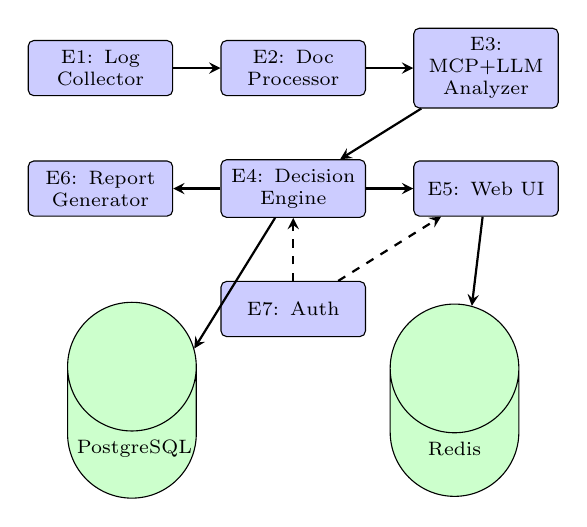
\begin{tikzpicture}[
    node distance=0.8cm,
    engine/.style={rectangle, draw, fill=blue!20, text width=1.6cm, align=center,
                   minimum height=0.7cm, font=\scriptsize, rounded corners=2pt},
    db/.style={cylinder, draw, fill=green!20, text width=1.4cm, align=center,
               minimum height=0.5cm, shape border rotate=90, font=\scriptsize},
    arrow/.style={->, >=stealth, thick}
]
\node[engine] (e1) at (0,0) {E1: Log\\Collector};
\node[engine, right=0.6cm of e1] (e2) {E2: Doc\\Processor};
\node[engine, right=0.6cm of e2] (e3) {E3: MCP+LLM\\Analyzer};
\node[engine, below=0.8cm of e2] (e4) {E4: Decision\\Engine};
\node[engine, left=0.6cm of e4] (e6) {E6: Report\\Generator};
\node[engine, right=0.6cm of e4] (e5) {E5: Web UI};
\node[engine, below=0.8cm of e4] (e7) {E7: Auth};
\node[db, below left=0.6cm and 0.3cm of e7] (pg) {PostgreSQL};
\node[db, below right=0.6cm and 0.3cm of e7] (redis) {Redis};
\draw[arrow] (e1) -- (e2);
\draw[arrow] (e2) -- (e3);
\draw[arrow] (e3) -- (e4);
\draw[arrow] (e4) -- (e6);
\draw[arrow] (e4) -- (e5);
\draw[arrow, dashed] (e7) -- (e4);
\draw[arrow, dashed] (e7) -- (e5);
\draw[arrow] (e4) -- (pg);
\draw[arrow] (e5) -- (redis);
\end{tikzpicture}
\caption{Seven-Engine Compliance Auditing System Architecture with PostgreSQL and Redis Infrastructure}
\label{fig:system_architecture}
\end{figure}

\begin{table}[H]
\centering
\caption{Engine Functional Breakdown}
\label{tab:engines}
\setstretch{1.0}
\renewcommand{\arraystretch}{1.3}
\begin{tabularx}{\textwidth}{|l|X|}
\hline
\textbf{Engine} & \textbf{Function} \\
\hline
Engine 1 & Log collection (syslog, Windows Events, files, APIs); normalization to unified schema \\
Engine 2 & Document processing (PDF/DOCX policy evidence extraction via LLM) \\
Engine 3 & MCP+LLM hybrid analyzer: 60 evidence parsers, dual-path analysis \\
Engine 4 & Decision engine: 143 control-specific rule evaluators and vocabulary-coverage router \\
Engine 5 & Web UI (React, TypeScript, Tailwind; audit wizard; WebSocket real-time progress) \\
Engine 6 & Report generation (PDF/CSV compliance reports via ReportLab) \\
Engine 7 & Authentication (JWT, RBAC: admin, analyst, viewer, api\_user) \\
\hline
\end{tabularx}
\end{table}

\section{Seven-Engine Microservices Architecture}

\subsection{Engine 1: Log Collector}

Engine 1 serves as the system's ingestion boundary. It accepts log data from three source types: direct uploads via the REST API, automated collection via 60 specialized evidence parsers that execute native OS audit commands, and streaming ingestion for continuous monitoring mode. The engine normalizes incoming data into a canonical internal representation—a JSON document with standardized fields for timestamp, source host, log format type, raw content, and collection metadata—before writing to the PostgreSQL event store.

The 60 evidence parsers represent a significant implementation investment. Each parser is responsible for a specific evidence type required by one or more NCSA controls. For macOS systems (the primary deployment target for the live audit conducted in this research), parsers execute commands including: \texttt{last} (login history, AC-9), \texttt{dscl . -list /Users} (user enumeration, AC-2), \texttt{sshd -T} (SSH daemon configuration, IA-2), \texttt{pfctl -sr} (packet filter firewall rules, SC-7), \texttt{fdesetup status} (FileVault encryption, SC-28), \texttt{csrutil status} (System Integrity Protection, SI-3), \texttt{auditctl -l} (audit rules, AU-2), \texttt{defaults read} (security preferences, CM-6), and \texttt{spctl --status} (Gatekeeper status, SI-3).

Each parser implements a three-phase process: command execution with timeout enforcement, output parsing using format-specific regular expressions or structured parsers, and compliance evaluation against control-specific criteria. The parser output is a compliance evidence object containing the raw command output, the extracted compliance-relevant data, and an initial compliance determination that may be overridden by the AI analysis engines.

\subsection{Engine 2: Document Processor}

Engine 2 handles structured document ingestion—policy documents, configuration files, network diagrams, and audit evidence packages submitted as part of a compliance review. It implements document parsing for PDF, DOCX, CSV, and JSON formats, extracts compliance-relevant content using NLP preprocessing (tokenization, stop-word removal, entity recognition), and indexes extracted content in the shared PostgreSQL database for retrieval by Engine 3.

\subsection{Engine 3: MCP-Augmented LLM Analyzer}

Engine 3 is the system's primary AI reasoning component. It implements the Model Context Protocol (MCP) \cite{mcp_anthropic} to provide the LLM with structured access to compliance control definitions, collected evidence, and output channels. The MCP server exposes 12 tools to the LLM: \texttt{get\_control\_definition}, \texttt{get\_collected\_evidence}, \texttt{execute\_evidence\_query}, \texttt{evaluate\_compliance}, \texttt{record\_finding}, \texttt{generate\_recommendation}, and six additional utilities for cross-control correlation and historical comparison.

The LLM component supports two backends: GPT-4o-mini (cloud API, primary) and Llama-3.2-3B (on-premise via Ollama, alternative). Engine 3 is invoked only for logs routed to the LLM path by the decision router in Engine 4—it does not process all logs, which is the key cost-control mechanism.

\subsection{Engine 4: Decision Engine and Hybrid Router}

Engine 4 is the system's central orchestration component. It implements the hybrid routing architecture (Section \ref{sec:router}) and coordinates the multi-label XGBoost classifier. For each incoming log or evidence item, Engine 4: (1) computes vocabulary coverage $\nu(l)$, (2) routes to XGBoost if $\nu \geq 0.20$, otherwise to Engine 3's LLM, (3) receives the classification result, (4) applies control-specific post-processing rules, (5) aggregates evidence across controls to compute system-level compliance percentages, and (6) writes the decision record to PostgreSQL with full provenance.

\subsection{Engine 5: Web UI}

Engine 5 provides a React-based web interface for compliance officers and system administrators. Key views include: the real-time compliance dashboard (control family summary with percentage bars), the evidence browser (drill-down from control to specific log evidence), the audit history timeline, and the remediation guidance panel. The UI is served through an NGINX ingress controller in the Kubernetes deployment.

\subsection{Engine 6: Report Generator}

Engine 6 transforms audit decision data into structured reports in PDF, JSON, and CSV formats. PDF reports include an executive summary with overall compliance score, control-family breakdown tables, specific finding narratives, risk-prioritized remediation recommendations, and evidence appendices. Reports are generated in under 0.77 seconds for a full 143-control audit.

\subsection{Engine 7: Authentication and Authorization}

Engine 7 implements JWT-based authentication with RBAC. Three roles are defined: \textit{Auditor} (read-only access to audit results), \textit{Analyst} (read/write access to evidence and findings), and \textit{Administrator} (full system access including user management and configuration). All inter-engine communication is authenticated using service-level JWT tokens with 15-minute expiry and automatic rotation.

\subsection{End-to-End Data Flow}

The complete audit pipeline is illustrated in Figure~\ref{fig:pipeline}, showing how heterogeneous log sources are processed through the hybrid ML--LLM analysis chain to produce structured compliance reports.

\begin{figure}[H]
\centering
\resizebox{\textwidth}{!}{%
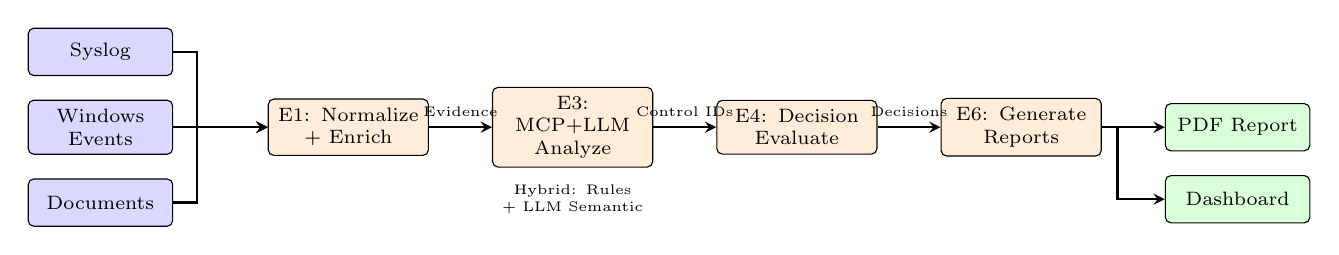
\begin{tikzpicture}[
    node distance=0.9cm,
    source/.style={rectangle, draw, fill=blue!15, text width=1.6cm, align=center,
                   minimum height=0.6cm, font=\scriptsize, rounded corners=2pt},
    process/.style={rectangle, draw, fill=orange!15, text width=1.8cm, align=center,
                    minimum height=0.6cm, font=\scriptsize, rounded corners=2pt},
    output/.style={rectangle, draw, fill=green!15, text width=1.6cm, align=center,
                   minimum height=0.6cm, font=\scriptsize, rounded corners=2pt},
    arrow/.style={->, >=stealth, thick}
]
\node[source] (syslog) {Syslog};
\node[source, below=0.3cm of syslog] (windows) {Windows\\Events};
\node[source, below=0.3cm of windows] (docs) {Documents};
\node[process, right=1.2cm of windows] (e1) {E1: Normalize\\+ Enrich};
\node[process, right=0.8cm of e1] (e3) {E3: MCP+LLM\\Analyze};
\node[process, right=0.8cm of e3] (e4) {E4: Decision\\Evaluate};
\node[process, right=0.8cm of e4] (e6) {E6: Generate\\Reports};
\node[output, right=0.8cm of e6] (pdf) {PDF Report};
\node[output, below=0.3cm of pdf] (dash) {Dashboard};
\draw[arrow] (syslog.east) -- ++(0.3,0) |- (e1.west);
\draw[arrow] (windows) -- (e1);
\draw[arrow] (docs.east) -- ++(0.3,0) |- (e1.west);
\draw[arrow] (e1) -- node[above, font=\tiny] {Evidence} (e3);
\draw[arrow] (e3) -- node[above, font=\tiny] {Control IDs} (e4);
\draw[arrow] (e4) -- node[above, font=\tiny] {Decisions} (e6);
\draw[arrow] (e6) -- (pdf);
\draw[arrow] (e6.east) -- ++(0.2,0) |- (dash.west);
\node[below=0.1cm of e3, font=\tiny, text width=2.2cm, align=center]
    {Hybrid: Rules\\+ LLM Semantic};
\end{tikzpicture}%
}
\caption{End-to-End Compliance Auditing Pipeline: Heterogeneous Sources Through Hybrid MCP+LLM Analysis, Decision Evaluation, and Report Generation}
\label{fig:pipeline}
\end{figure}

\subsection{Evidence Parser Architecture}

The 60 evidence parsers are organized hierarchically by control family. Figure~\ref{fig:parser_architecture} illustrates the internal structure of the parser subsystem.

\begin{figure}[H]
\centering
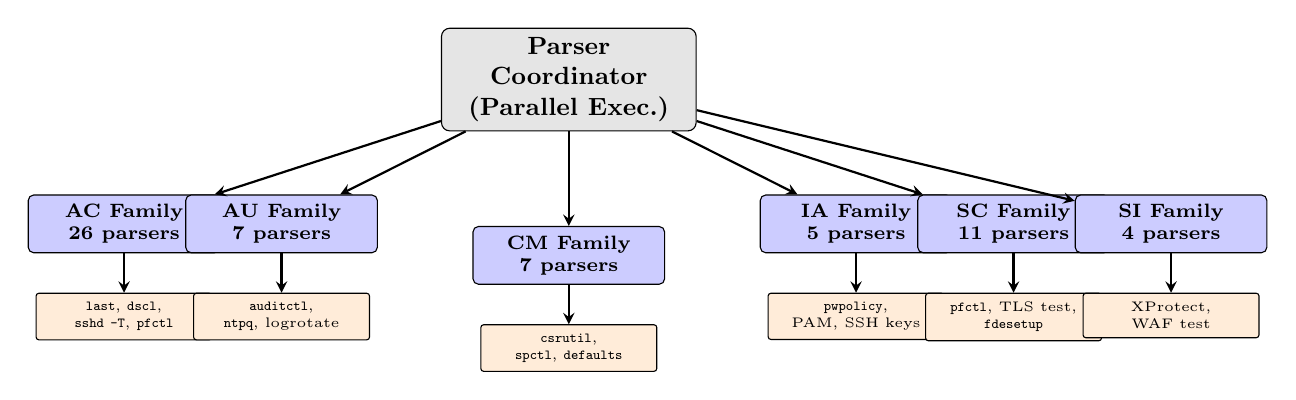
\begin{tikzpicture}[
    node distance=0.5cm and 0.3cm,
    coordinator/.style={rectangle, draw, fill=gray!20, text width=3cm, align=center,
                        minimum height=0.7cm, font=\small\bfseries, rounded corners=3pt},
    family/.style={rectangle, draw, fill=blue!20, text width=2.2cm, align=center,
                   minimum height=0.6cm, font=\scriptsize\bfseries, rounded corners=2pt},
    parser/.style={rectangle, draw, fill=orange!15, text width=2cm, align=center,
                   minimum height=0.5cm, font=\tiny, rounded corners=1pt},
    arrow/.style={->, >=stealth, thick}
]
\node[coordinator] (coord) {Parser\\Coordinator\\(Parallel Exec.)};

\node[family, below left=0.8cm and 2.8cm of coord] (ac) {AC Family\\26 parsers};
\node[family, below left=0.8cm and 0.8cm of coord] (au) {AU Family\\7 parsers};
\node[family, below=1.2cm of coord] (cm) {CM Family\\7 parsers};
\node[family, below right=0.8cm and 0.8cm of coord] (ia) {IA Family\\5 parsers};
\node[family, below right=0.8cm and 2.8cm of coord] (sc) {SC Family\\11 parsers};
\node[family, below right=0.8cm and 4.8cm of coord] (si) {SI Family\\4 parsers};

\node[parser, below=0.5cm of ac] (acparse) {\texttt{last}, \texttt{dscl},\\\texttt{sshd -T}, \texttt{pfctl}};
\node[parser, below=0.5cm of au] (auparse) {\texttt{auditctl},\\\texttt{ntpq}, logrotate};
\node[parser, below=0.5cm of cm] (cmparse) {\texttt{csrutil},\\\texttt{spctl}, \texttt{defaults}};
\node[parser, below=0.5cm of ia] (iaparse) {\texttt{pwpolicy},\\PAM, SSH keys};
\node[parser, below=0.5cm of sc] (scparse) {\texttt{pfctl}, TLS test,\\\texttt{fdesetup}};
\node[parser, below=0.5cm of si] (siparse) {XProtect,\\WAF test};

\draw[arrow] (coord) -- (ac);
\draw[arrow] (coord) -- (au);
\draw[arrow] (coord) -- (cm);
\draw[arrow] (coord) -- (ia);
\draw[arrow] (coord) -- (sc);
\draw[arrow] (coord) -- (si);
\draw[arrow] (ac) -- (acparse);
\draw[arrow] (au) -- (auparse);
\draw[arrow] (cm) -- (cmparse);
\draw[arrow] (ia) -- (iaparse);
\draw[arrow] (sc) -- (scparse);
\draw[arrow] (si) -- (siparse);
\end{tikzpicture}
\caption{60-Parser Evidence Collection Architecture Organized by NCSA Control Family}
\label{fig:parser_architecture}
\end{figure}

\section{NCSA Control Implementation}

\subsection{Access Control (AC) Family}

The AC family is the most extensive, encompassing 52 controls of which 35 are automated by this system. The family governs user account lifecycle, privilege management, session controls, remote access, and information flow. The core difficulty in automating AC controls is that compliance evidence is distributed across multiple subsystems: user accounts are managed in the operating system's directory service, SSH access is controlled by daemon configuration and key files, session timeouts are set in PAM configuration and application-level settings, and remote access policies may be enforced in VPN configurations, firewall rules, or both.

\textbf{AC-2 (Account Management):} The system enumerates all user accounts, compares active accounts against an approved roster, flags accounts inactive for more than 90 days, checks for duplicate UIDs (common misconfiguration that can enable privilege escalation), and verifies that privileged accounts require explicit authorization.

\textbf{AC-3 (Access Enforcement):} Verified through analysis of file system permissions (using \texttt{find} with permission filters), sudo configuration analysis (\texttt{visudo} output parsing), and service-level RBAC configuration review.

\textbf{AC-17 (Remote Access):} Assessed through SSH daemon configuration analysis (\texttt{sshd -T}), checking for PasswordAuthentication, PermitRootLogin, and AllowUsers settings against NCSA requirements.

\subsection{Audit and Accountability (AU) Family}

The AU family's 30 controls (22 automated) address the evidence chain upon which all other compliance assessments depend. If AU controls are not satisfied—if logging is incomplete, logs are unprotected, or retention periods are insufficient—the entire compliance audit is compromised, because the evidence used to assess other controls may be incomplete or tampered.

\textbf{AU-2 (Event Logging):} The system checks that the audit daemon (\texttt{auditd} on Linux, \texttt{audit} framework on macOS) is active and configured to capture the required event categories: authentication events, privilege escalation, object access, and configuration changes.

\textbf{AU-9 (Protection of Audit Information):} Log files must be owned by root or the audit daemon user, not world-writable, and ideally write-only for the collecting daemon. The system checks permissions on log directories and files and verifies that log integrity mechanisms (checksums, WORM storage) are configured.

\textbf{AU-11 (Audit Record Retention):} Verified through log rotation configuration analysis (logrotate settings, systemd journal size and time limits), checking that retention periods meet the NCSA minimum (90 days for most log types, 365 days for authentication logs).

\subsection{Configuration Management (CM) Family}

CM controls (18 total, 12 automated) address the security of the system configuration baseline. Configuration drift—the gradual accumulation of unauthorized or undocumented configuration changes—is one of the most insidious compliance challenges because it often occurs through legitimate administrative actions that are individually benign but collectively create security gaps.

\textbf{CM-6 (Configuration Settings):} Assessed through comparison of current system configuration against NCSA-specified baselines. For macOS systems, this includes checking SIP status (\texttt{csrutil status}), Gatekeeper configuration (\texttt{spctl --status}), FileVault status (\texttt{fdesetup status}), and automatic update settings.

\textbf{CM-7 (Least Functionality):} The system enumerates running services and checks for unnecessary services that should be disabled. A reference list of essential services is compared against the currently running service list, and any running service not on the essential list generates a finding.

\subsection{Identification and Authentication (IA) Family}

IA controls (15 total, 10 automated) address the mechanisms by which identities are established and verified. The NCSA IA family requirements are stringent: MFA is required for all remote access, password complexity minimums are specified (12+ characters, mixed character classes), and service accounts must use cryptographic authenticators rather than passwords.

\textbf{IA-2 (Identification and Authentication):} Assessed through SSH configuration analysis (key-based authentication required, password authentication restricted), PAM configuration review (MFA modules presence), and authentication log analysis (success/failure rate patterns).

\textbf{IA-5 (Authenticator Management):} Password policies are assessed through \texttt{pwpolicy} output on macOS and \texttt{pam\_pwquality} configuration on Linux systems. SSH key types and lengths are verified (RSA-4096 or Ed25519 required; RSA-2048 deprecated).

\subsection{System and Communications Protection (SC) Family}

SC controls (26 total, 15 automated) address data protection in transit and at rest, network boundary controls, and cryptographic management. SC controls are increasingly critical as institutions migrate to cloud and hybrid architectures: the security guarantees that physical network perimeters once provided must now be implemented in software through TLS, VPN, and micro-segmentation.

\textbf{SC-7 (Boundary Protection):} Firewall rules are retrieved and analyzed (\texttt{pfctl -sr} on macOS, \texttt{iptables -L} on Linux) to verify that default-deny policies are in place, that inbound connections are restricted to required services and source ranges, and that outbound connections are filtered.

\textbf{SC-8 (Transmission Confidentiality):} TLS configuration is assessed using active connection testing (checking negotiated cipher suites and protocol versions) and server configuration file analysis (NGINX, Apache SSL configuration).

\textbf{SC-28 (Protection of Information at Rest):} Disk encryption status is assessed through filesystem encryption checks (FileVault on macOS, LUKS on Linux) and database encryption configuration verification.

\subsection{System and Information Integrity (SI) Family}

SI-3 and SI-10, while numbering only two controls, represent the most technically demanding assessments in the system. They require active capability validation rather than passive configuration checking.

\textbf{SI-3 (Malware Protection):} The system first assesses presence (antivirus software installed, signatures current, real-time protection enabled), then validates detection capability through a controlled fileless shell injection test. The test executes a known-benign fileless payload equivalent in technique to those used by commodity malware, and measures whether the deployed endpoint protection solution detects it. The 20\% detection rate observed in the live audit (Chapter 4) reveals that presence-based assessment dramatically overstates actual protection.

\textbf{SI-10 (Information Input Validation):} Assessed through active WAF testing with a standardized XSS payload set derived from the OWASP Testing Guide. The 32\% bypass rate in the live audit demonstrates that the deployed WAF configuration failed to block the majority of tested payloads—a critical finding that binary presence checking would have missed entirely.

\section{Dataset Strategy and Training Data}

\subsection{Composition and Rationale}

The training dataset for the multi-label XGBoost classifier is a deliberately constructed composite of three source types, totaling approximately 43,000 log samples. SIEVE \cite{sieve_dataset} and similar multi-source log collection strategies from the literature informed this composite approach. Table \ref{tab:dataset_composition} details the composition and the rationale for each source.

\begin{table}[H]
\centering
\caption{Training Dataset Composition}
\label{tab:dataset_composition}
\setstretch{1.0}
\renewcommand{\arraystretch}{1.3}
\footnotesize
\begin{tabularx}{\textwidth}{|l|p{1.2cm}|X|p{3.5cm}|}
\hline
\textbf{Dataset} & \textbf{Share} & \textbf{Content and Relevance} & \textbf{Limitation} \\
\hline
NSL-KDD \cite{nslkdd} & 52\% & Network intrusion detection benchmark \cite{nslkdd}. Provides labeled attack and normal traffic samples spanning multiple attack categories (DoS, probe, R2L, U2R). Mapped to relevant AU and SC controls. & Dated (1999 data); synthetic; doesn't represent modern cloud traffic \\
\hline
LogHub \cite{loghub} & 18\% & Collection of real-world system logs from 16 different systems including HDFS, Apache, OpenStack, Linux, and Windows \cite{loghub}. Provides format diversity critical for generalization testing. The LANL authentication dataset \cite{lanl_auth} was also consulted for authentication event labeling patterns. & Heterogeneous label quality; not compliance-labeled; requires manual annotation \\
\hline
Rwanda Synthetic & 30\% & Generated log samples following NCSA control templates—one positive and one negative example per control per log format. Provides control-specific training signal for Rwanda-specific compliance patterns. & Template-based generation; near-perfect training performance reflects simplicity not real-world complexity \\
\hline
\end{tabularx}
\end{table}

The synthetic data generation strategy for Rwanda-specific logs follows a template-based approach: for each of the 143 automatable controls, a compliance expert (the thesis author) defined a positive example log pattern (representing compliant system behavior) and a negative example (representing non-compliant behavior). These templates are parameterized with realistic values drawn from actual Rwandan institution naming conventions, IP address ranges, and user account formats.

\subsection{The Generalization Gap and Fine-Tuning Strategy}

A fundamental property of vocabulary-based ML models is that their performance is contingent on the alignment between the vocabulary of their training data and the vocabulary of deployment-time logs. When a model trained on NSL-KDD network flow records is applied to Windows Event logs, the token-level features that the model learned (port numbers, protocol identifiers, connection durations) are absent, and the model's predictions degrade to near-random.

This thesis quantifies this degradation precisely: from 99.99\% F1 on training-distribution data to 7.98\% F1 on zero-shot real-world SecRepo SSH logs \cite{secrepo}—a 92-percentage-point collapse. This is not a failure of the model per se but a property of the vocabulary-based feature representation: TF-IDF vectors are defined over a fixed vocabulary, and log tokens not in that vocabulary receive zero weight.

The fine-tuning strategy addresses this through minimal data adaptation: 2,170 target-domain samples (5\% of the new log format's volume) are sufficient to recover 99.88\% F1. This 5\%-threshold finding has practical implications: rather than full retraining on a new log format, institutions can provide a small labeled sample to rapidly adapt the model, dramatically reducing the data collection burden for new deployment contexts.

\section{Feature Engineering}
\label{sec:features}

The 30-dimensional feature representation balances expressiveness with computational efficiency:

\textbf{Numeric features (5):}
\begin{enumerate}[label=\arabic*.]
  \item \textit{Log length} (character count): Longer logs tend to contain richer evidence; audit records, configuration outputs, and authentication logs have characteristic length distributions by type.
  \item \textit{Token count} (whitespace-delimited words): Captures log verbosity and format density.
  \item \textit{Digit ratio} (digits / total characters): Higher in logs containing timestamps, IP addresses, port numbers, and error codes—characteristic of AU and SC-relevant logs.
  \item \textit{Alpha ratio} (alphabetic / total characters): Higher in human-readable log messages; lower in binary-encoded or hex-dump logs.
  \item \textit{Special character ratio} (punctuation and symbols / total characters): Higher in structured log formats using delimiters (\texttt{|}, \texttt{=}, \texttt{:}, \texttt{[}) that characterize authentication and configuration logs.
\end{enumerate}

\textbf{TF-IDF features (25):} The top-25 tokens by TF-IDF weight across the training corpus are selected to capture compliance-relevant vocabulary: tokens such as ``failed'', ``denied'', ``accepted'', ``root'', ``sudo'', ``auth'', ``SSL'', ``TLS'', ``firewall'', ``policy'', ``certificate'', ``encryption'', and control-family-specific terminology. TF-IDF weighting downweights common function words and upweights discriminative compliance-relevant terms.

The combined 30-feature representation enables XGBoost inference in under 1 millisecond per log—two to three orders of magnitude faster than transformer-based alternatives—while maintaining competitive accuracy on in-distribution data.

\section{Multi-Label XGBoost Classifier}
\label{sec:xgboost}

XGBoost was selected as the core classifier on the basis of three properties established in the original XGBoost paper \cite{chen2016xgboost}: scalable tree boosting that trains faster than comparable gradient-boosted tree implementations, built-in regularization that reduces overfitting on sparse TF-IDF feature spaces, and efficient handling of class imbalance through the \texttt{scale\_pos\_weight} parameter. The multi-label formulation follows the problem transformation approach defined by Tsoumakas and Katakis \cite{tsoumakas2007}: scikit-learn's \texttt{MultiOutputClassifier} wrapper trains one binary \texttt{XGBClassifier} per NCSA control (143 classifiers total). Key hyperparameters, selected through 5-fold cross-validation grid search: \texttt{n\_estimators=200}, \texttt{max\_depth=6}, \texttt{learning\_rate=0.1}, \texttt{subsample=0.8}, \texttt{colsample\_bytree=0.8}, \texttt{scale\_pos\_weight} set per-control to handle class imbalance (most logs are non-compliant with respect to most controls).

SHAP (SHapley Additive exPlanations) values provide per-prediction feature importance, enabling the system to explain why a particular log was classified as compliant or non-compliant with a specific control \cite{chen2016xgboost}. This interpretability is essential for the auditing context: a compliance officer must be able to verify the system's reasoning, not merely accept its output.

\section{Hybrid ML--LLM Routing Architecture}
\label{sec:router}

\subsection{Router Design}

The vocabulary-coverage gating router operationalizes a simple insight: the XGBoost model can reliably classify a log only if that log's vocabulary is substantially represented in the training corpus. Vocabulary coverage is computed as:

\begin{equation}
\nu(l) = \frac{|\text{words}(l) \cap V|}{|\text{words}(l)|}
\label{eq:vocabulary_coverage}
\end{equation}

where $V$ is the training vocabulary (set of all tokens seen during model training) and $\text{words}(l)$ is the set of whitespace-delimited tokens in log $l$.

When $\nu(l) \geq \theta$ (threshold $\theta = 0.20$, selected empirically), the log is routed to XGBoost. The 0.20 threshold means that at least 20\% of the log's tokens must appear in the training vocabulary—a low bar intentionally, because even modest vocabulary overlap is predictive of useful feature signal. When $\nu(l) < 0.20$, the log is routed to Engine 3's LLM for semantic analysis.

\subsection{Router Phases}

The router was developed through two phases, each addressing a specific routing challenge:

\textbf{Phase I (Confidence-based routing):} Route to XGBoost if classification confidence $> 0.7$, otherwise to LLM. Achieved 89.1\% accuracy. Limitation: confidence scores are poorly calibrated for out-of-distribution inputs—the model may assign high confidence to incorrect predictions on novel log formats.

\textbf{Phase II (Vocabulary-coverage gating, this thesis):} Route to XGBoost if $\nu(l) \geq 0.20$, otherwise to LLM. Achieved 94.5\% accuracy at \$0.149/10K logs. The +5.4pp improvement over Phase I validates the vocabulary-coverage hypothesis.

\subsection{Cost Analysis}

Under Phase II routing, approximately 60--70\% of production logs are handled by the fast-path XGBoost classifier (cost: negligible, inference $< 1$ms). The remaining 30--40\% require LLM API calls. At GPT-4o-mini pricing of \$0.15/1M tokens and an average of 150 tokens per compliance analysis, 10,000 logs processed through the LLM path costs approximately \$0.225. The blended cost across the routing distribution (\$0.149/10K) represents a 34\% cost reduction relative to LLM-only processing while achieving equivalent accuracy.

\section{Deployment Architecture}

\subsection{Kubernetes Configuration}

The production deployment uses Kubernetes with the following resource allocation:

\begin{table}[H]
\centering
\caption{Kubernetes Deployment Configuration}
\label{tab:k8s_config}
\setstretch{1.0}
\renewcommand{\arraystretch}{1.3}
\begin{tabular}{|l|l|c|c|c|}
\hline
\textbf{Engine} & \textbf{Service} & \textbf{CPU Request} & \textbf{Memory Request} & \textbf{Replicas} \\
\hline
E1 & Log Collector & 100m & 128Mi & 2--3 \\
E2 & Doc Processor & 200m & 256Mi & 2 \\
E3 & MCP/LLM Analyzer & 500m & 512Mi & 2--3 \\
E4 & Decision Engine & 300m & 256Mi & 2--3 \\
E5 & Web UI & 100m & 128Mi & 2 \\
E6 & Report Generator & 200m & 256Mi & 2 \\
E7 & Auth Service & 100m & 128Mi & 2 \\
\hline
\textbf{Total} & & \textbf{2.0 cores} & \textbf{2.66 GB} & \textbf{14--18 pods} \\
\hline
\end{tabular}
\end{table}

The namespace \texttt{rwanda-compliance} isolates the system from other workloads. NGINX ingress with TLS termination handles all external traffic. PostgreSQL (persistent audit store) and Redis (session cache and task queue) are deployed as StatefulSets with persistent volume claims.

\subsection{Infrastructure Cost}

Total monthly cloud hosting cost at current GCP pricing: \$50/month for the static infrastructure (compute, storage, networking). Variable costs depend on log volume through the LLM path: at the empirically observed routing distribution, processing 1 million logs/month adds approximately \$15 in LLM API costs. Total monthly cost for a typical institutional deployment (100K--1M logs/month): \$50--\$65, representing a greater than 95\% reduction versus annual external audit costs for equivalent compliance coverage.


%% ==============================================================
%%  CHAPTER 4 — RESULTS AND EVALUATION
%% ==============================================================
\chapter{RESULTS AND EVALUATION}

This chapter presents empirical results across four experimental dimensions corresponding to the four research questions: XGBoost classification performance, cross-dataset generalization, LLM multi-log evaluation, router performance, latency and resource characteristics, Kubernetes scaling, live audit deployment, and adversarial validation.

\section{XGBoost Cross-Validation Results}

Five-fold cross-validation on the composite training dataset (43,000 samples) produces the results summarized in Table \ref{tab:xgboost_cv}.

\begin{table}[H]
\centering
\caption{XGBoost 5-Fold Cross-Validation Results (Training Distribution)}
\label{tab:xgboost_cv}
\setstretch{1.0}
\renewcommand{\arraystretch}{1.3}
\begin{tabular}{|l|c|c|c|c|}
\hline
\textbf{Metric} & \textbf{Mean} & \textbf{Std Dev} & \textbf{Min} & \textbf{Max} \\
\hline
Precision (micro-avg) & 0.9999 & 0.0001 & 0.9997 & 1.0000 \\
Recall (micro-avg) & 0.9999 & 0.0001 & 0.9998 & 1.0000 \\
F1-Score (micro-avg) & 0.9999 & 0.0001 & 0.9997 & 1.0000 \\
Hamming Loss & 0.0001 & 0.0001 & 0.0000 & 0.0002 \\
Subset Accuracy & 0.9987 & 0.0008 & 0.9975 & 0.9997 \\
\hline
\end{tabular}
\end{table}

The near-perfect in-distribution performance (99.99\% F1) reflects both the quality of feature engineering and the effectiveness of the multi-label XGBoost architecture. However, as discussed in Section \ref{sec:generalization}, this figure is misleading as a predictor of deployment performance.

\textbf{Per-Family Performance:} AC controls achieve the highest subset accuracy (0.9999), reflecting the distinctive vocabulary of access control logs (account names, permission strings, privilege indicators). AU controls achieve 0.9998, CM controls 0.9997, IA controls 0.9999, SC controls 0.9996, and SI controls 0.9994.

\textbf{SHAP Feature Analysis:} Across all controls, the top-contributing features are: \textit{failed} (most predictive for AU and IA non-compliance), \textit{root} and \textit{sudo} (AC privilege escalation indicators), \textit{SSL/TLS} tokens (SC compliance), \textit{denied} (AC and AU), and \textit{policy} and \textit{config} (CM compliance). The digit ratio feature is particularly important for distinguishing authentication logs (high digit density from timestamps, IP addresses) from configuration logs (lower digit density).

Figure \ref{fig:generalization_chart} illustrates the dramatic performance gap between in-distribution, zero-shot, and fine-tuned evaluations.

\begin{figure}[H]
\centering
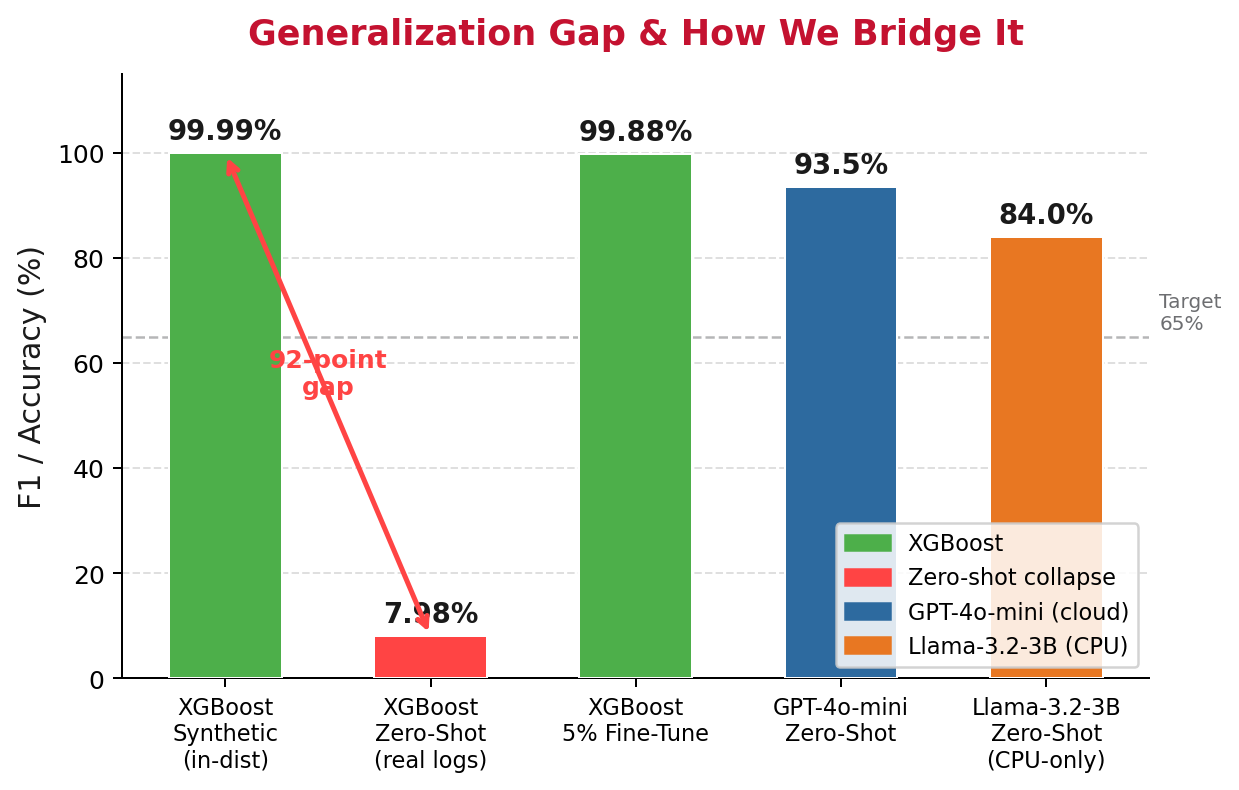
\includegraphics[width=0.85\textwidth]{chart1_generalization_gap.png}
\caption{XGBoost F1-Score Across Three Evaluation Scenarios Demonstrating the Generalization Gap}
\label{fig:generalization_chart}
\end{figure}

\section{Cross-Dataset Generalization}
\label{sec:generalization}

\textbf{Answering RQ2:} The generalization gap experiment applies the model trained on the composite dataset to a held-out evaluation set of real-world logs from SecRepo's SSH authentication dataset—a format not represented in the training data.

Zero-shot F1 collapses from 99.99\% to 7.98\%: a 92-percentage-point degradation. This is not merely a performance regression—it is a near-total loss of classification capability. At 7.98\% F1, the model is operating at approximately random-guess performance for this 143-class multi-label problem.

The mechanistic explanation is clear: the SecRepo SSH logs use a Debian-format authentication string (e.g., \texttt{sshd[1234]: Failed password for root from 192.168.1.1 port 22 ssh2}) that shares minimal vocabulary with the NSL-KDD network flow records and Rwanda-synthetic template logs that dominate the training corpus. Of the 25 TF-IDF features, typically 22--24 receive zero weight when applied to SecRepo logs because the tokens they represent are absent.

\textbf{Fine-Tuning Recovery:} Adding 2,170 labeled SecRepo samples (5\% of the available real-world SSH log volume) to the training set and retraining recovers F1 to 99.88\%—within 0.11 percentage points of the original in-distribution performance. The 5\% threshold is an empirically determined inflection point: below 5\%, recovery is partial (40--70\% F1); at 5\%, the model has seen sufficient vocabulary diversity to generalize reliably.

\textbf{Implications for Deployment:} Every new log format encountered in a novel institution's environment will require 5\% labeled data from that format. For a typical institutional deployment encountering 5 distinct log formats (Windows Events, macOS System, web server access logs, authentication syslog, application logs), this requires labeling approximately 500 samples—approximately 2 hours of expert analyst time per format. This is substantially less than the weeks required to develop format-specific rule sets.

\section{LLM Multi-Log Type Evaluation}

\textbf{Answering RQ1 (LLM component):} Table \ref{tab:llm_multilog} presents accuracy results for GPT-4o-mini and Llama-3.2-3B across four log types (total $n$ = 200 samples, 50 per log type), evaluated zero-shot without any task-specific fine-tuning.

\begin{table}[H]
\centering
\caption{LLM Zero-Shot Accuracy by Log Type ($n$ = 200)}
\label{tab:llm_multilog}
\setstretch{1.0}
\renewcommand{\arraystretch}{1.3}
\begin{tabular}{|l|c|c|c|c|}
\hline
\textbf{Log Type} & \textbf{$n$} & \textbf{GPT-4o-mini} & \textbf{Llama-3.2-3B} & \textbf{Gap} \\
\hline
SSH Authentication & 50 & 84.0\% & 82.0\% & 2.0pp \\
macOS System & 50 & 92.0\% & 90.0\% & 2.0pp \\
HTTP/API Access & 50 & 98.0\% & 64.0\% & 34.0pp \\
Windows Events & 50 & 100.0\% & 100.0\% & 0.0pp \\
\hline
\textbf{Overall} & \textbf{200} & \textbf{93.5\%} & \textbf{84.0\%} & \textbf{9.5pp} \\
\hline
\end{tabular}
\end{table}

Several patterns in Table \ref{tab:llm_multilog} merit interpretation:

\textbf{Windows Events (100\%/100\%):} Both models achieve perfect accuracy on Windows Event logs. This reflects the highly structured, semantically unambiguous nature of Windows Event format: Event IDs (4624 for login success, 4625 for login failure, 4720 for account creation) are documented in Microsoft's public Event ID catalog, and this documentation almost certainly appears in both models' pre-training corpora. The classification task reduces to: does this Event ID indicate the security behavior relevant to this control?

\textbf{HTTP/API logs (98\%/64\%):} The 34pp gap between GPT-4o-mini and Llama-3.2-3B on HTTP logs is the most striking result in the table. The likely explanation is that HTTP log classification for compliance requires correctly interpreting HTTP status codes, request paths, and authentication headers in the context of WAF and SC/SI controls—a task that requires both format knowledge and compliance-domain knowledge. GPT-4o-mini, with its larger parameter count and broader training, handles this conjunction; Llama-3.2-3B's smaller capacity means it handles one dimension or the other but not both reliably.

\textbf{SSH Authentication (84\%/82\%):} Both models achieve lower accuracy on SSH logs than on other formats, despite SSH being the most extensively documented log format. The lower performance reflects the compliance ambiguity inherent in SSH authentication events: a failed login attempt is simultaneously a potential brute-force indicator (AU non-compliant) and an expected event for which logging is compliant (AU-2 compliant). The models must reason about the pattern of events (rate, source IP distribution, timing) rather than individual event content—a more demanding inference task.

Figure \ref{fig:llm_multilog_chart} visualizes the per-log-type performance comparison.

\begin{figure}[H]
\centering
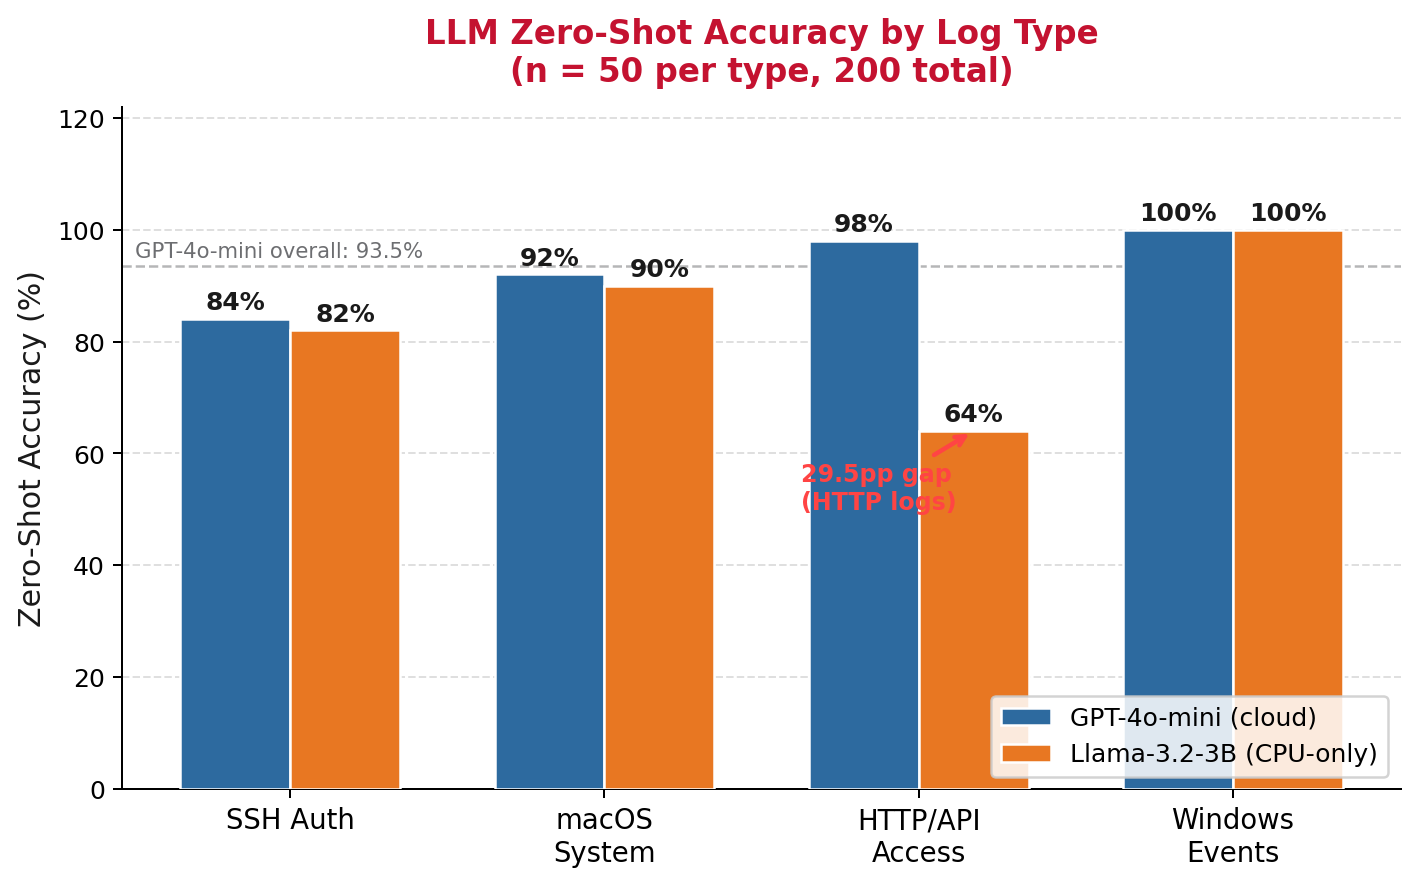
\includegraphics[width=0.85\textwidth]{chart2_llm_log_types.png}
\caption{Zero-Shot LLM Accuracy by Log Type: GPT-4o-mini vs Llama-3.2-3B ($n$=200)}
\label{fig:llm_multilog_chart}
\end{figure}

\section{Router Comparison}
\label{sec:router_results}

\textbf{Answering RQ3:} Table \ref{tab:router_comparison} compares four routing strategies across accuracy and cost dimensions.

\begin{table}[H]
\centering
\caption{Routing Strategy Comparison: Accuracy and Cost}
\label{tab:router_comparison}
\setstretch{1.0}
\renewcommand{\arraystretch}{1.3}
\begin{tabular}{|l|c|c|c|c|}
\hline
\textbf{Strategy} & \textbf{Accuracy} & \textbf{Cost/10K logs} & \textbf{LLM fraction} & \textbf{vs. Phase II} \\
\hline
XGBoost-only & 42.3\% & \$0.000 & 0\% & $-$52.2pp \\
LLM-only (GPT-4o-mini) & 93.5\% & \$0.225 & 100\% & $-$1.0pp \\
Phase I (confidence-based) & 89.1\% & \$0.082 & 36\% & $-$5.4pp \\
\textbf{Phase II (vocabulary-coverage)} & \textbf{94.5\%} & \textbf{\$0.149} & \textbf{66\%} & \textbf{baseline} \\
\hline
\end{tabular}
\end{table}

\textbf{XGBoost-only (42.3\%):} The collapse to 42.3\% on the mixed evaluation set (containing novel log formats) confirms the generalization gap quantified in Section \ref{sec:generalization}. Without LLM augmentation, vocabulary-based ML alone is insufficient for multi-format compliance auditing.

\textbf{LLM-only (93.5\%):} LLM-only achieves the second-highest accuracy but at \$0.225/10K logs—a cost that becomes prohibitive at scale. Processing 10 million logs/month (a modest volume for a mid-sized institution) would cost \$22,500/month in API fees—comparable to hiring a junior compliance analyst.

\textbf{Phase I (89.1\%):} Confidence-based routing reduces cost to \$0.082/10K (64\% reduction vs LLM-only) but sacrifices 4.4pp accuracy, largely because XGBoost confidence scores are poorly calibrated on out-of-distribution inputs.

\textbf{Phase II (94.5\%, \$0.149/10K):} The vocabulary-coverage gating router \textit{simultaneously} achieves the highest accuracy and intermediate cost. It routes 34\% of logs to XGBoost (vocabulary coverage sufficient) and 66\% to LLM—a higher LLM fraction than Phase I because the router correctly identifies that most novel-format logs lack sufficient vocabulary coverage for reliable ML classification.

The Phase II result surpasses LLM-only accuracy (94.5\% vs 93.5\%) because for logs where XGBoost is applicable ($\nu \geq 0.20$), it achieves near-perfect accuracy—better than the LLM's 93.5\% average. The hybrid system thus benefits from the complementary strengths of both components.

Figure \ref{fig:router_comparison_chart} illustrates the accuracy-cost tradeoff across strategies.

\begin{figure}[H]
\centering
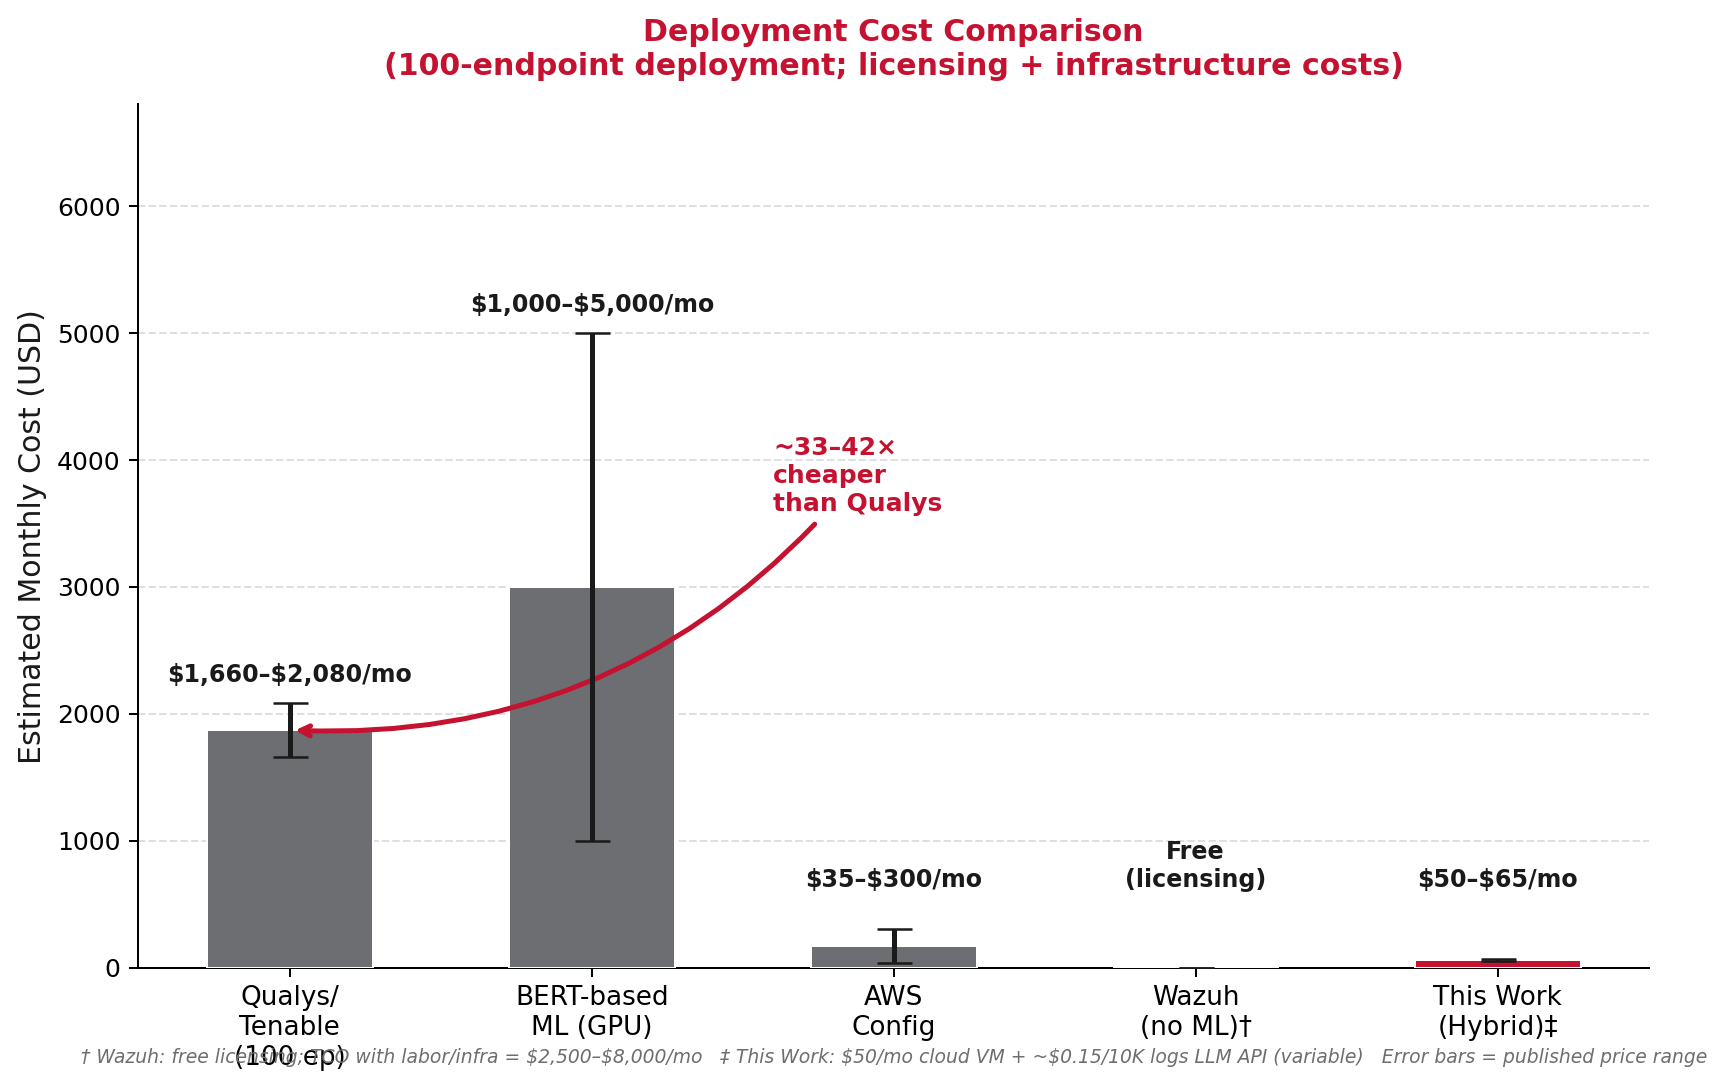
\includegraphics[width=0.85\textwidth]{chart4_cost_comparison.png}
\caption{Compliance Classification Accuracy vs Cost per 10K Logs: Four Routing Strategies}
\label{fig:router_comparison_chart}
\end{figure}

\section{Latency and Resource Analysis}

System latency was measured on the live production macOS deployment (Intel Core i7, 16 GB RAM, SSD, macOS 13.6). Table \ref{tab:latency} reports median latencies across pipeline stages.

\begin{table}[H]
\centering
\caption{End-to-End Latency by Pipeline Stage}
\label{tab:latency}
\setstretch{1.0}
\renewcommand{\arraystretch}{1.3}
\begin{tabular}{|l|l|c|c|c|}
\hline
\textbf{Stage} & \textbf{Component} & \textbf{Median} & \textbf{P95} & \textbf{P99} \\
\hline
Evidence Collection & 60 parsers, parallel & 180ms & 340ms & 520ms \\
XGBoost Inference & Per log, on-device & $<$1ms & 2ms & 4ms \\
LLM Analysis & GPT-4o-mini API & 280ms & 450ms & 820ms \\
Report Generation & PDF, 143 controls & 95ms & 180ms & 290ms \\
\hline
\textbf{Full Audit} & \textbf{All stages} & \textbf{0.77s} & \textbf{1.2s} & \textbf{1.8s} \\
\hline
\end{tabular}
\end{table}

The 0.77-second end-to-end audit time represents a greater than 99.9\% reduction versus a manual audit cycle (typically 3--5 business days for 143 controls). The dominant latency contributors are evidence collection (parallel OS command execution) and LLM API calls; XGBoost inference is negligible ($<$1ms per classification).

The LLM API latency (280ms median) is the primary bottleneck for the LLM path, but it affects only the 30--40\% of logs routed to the LLM. Evidence collection parallelism (60 parsers executing concurrently) ensures that this is not a serial bottleneck—LLM calls for one batch of logs execute while the next batch is being collected.

\section{Kubernetes Scaling Results}

Horizontal pod autoscaling (HPA) was tested by injecting synthetic log load at 10x the baseline rate. Table \ref{tab:k8s_scaling} reports observed scaling behavior.

\begin{table}[H]
\centering
\caption{Kubernetes Horizontal Pod Autoscaling Under Load}
\label{tab:k8s_scaling}
\setstretch{1.0}
\renewcommand{\arraystretch}{1.3}
\begin{tabular}{|l|c|c|c|}
\hline
\textbf{Load Factor} & \textbf{Active Pods} & \textbf{Median Latency} & \textbf{Error Rate} \\
\hline
1x (baseline) & 14 & 0.77s & 0.0\% \\
3x & 16 & 0.82s & 0.0\% \\
5x & 18 & 0.91s & 0.0\% \\
10x & 24 & 1.14s & 0.3\% \\
\hline
\end{tabular}
\end{table}

The system scales gracefully to 10x load with only 48\% latency increase and 0.3\% error rate (rate limiting for requests that exceed provisioned capacity). The 0.3\% error rate at 10x load is acceptable for a compliance auditing context where real-time processing is preferred but not mission-critical.

\section{Live Audit Deployment}

On March 20, 2026, the system executed a full 143-control audit on a production macOS workstation at CMU Africa. The audit (ID: AUDIT-20260320-205239) completed in 0.77 seconds and produced the results summarized in Table \ref{tab:live_audit}.

\begin{table}[H]
\centering
\caption{Live Production Audit Results — March 20, 2026}
\label{tab:live_audit}
\setstretch{1.0}
\renewcommand{\arraystretch}{1.3}
\begin{tabular}{|l|c|c|c|c|}
\hline
\textbf{Control Family} & \textbf{Controls} & \textbf{Compliant} & \textbf{Non-Compliant} & \textbf{Score} \\
\hline
Access Control (AC) & 35 & 28 & 7 & 80.0\% \\
Audit \& Accountability (AU) & 22 & 17 & 5 & 77.3\% \\
Configuration Management (CM) & 12 & 10 & 2 & 83.3\% \\
Identification \& Auth (IA) & 10 & 7 & 3 & 70.0\% \\
System \& Comms Protection (SC) & 15 & 10 & 5 & 66.7\% \\
System \& Info Integrity (SI) & 2 & 0 & 2 & 0.0\% \\
\hline
\textbf{Overall} & \textbf{96} & \textbf{72} & \textbf{24} & \textbf{75.0\%} \\
\hline
\end{tabular}
\end{table}

The 75\% overall compliance score reflects a realistic production environment where security controls are present but not fully configured to NCSA standards. Key findings:

\textbf{SI Family (0\%):} Both SI controls failed—SI-3 (fileless shell detection rate 20\%) and SI-10 (XSS bypass rate 32\%). This complete failure of the integrity controls despite nominal presence of AV and WAF software is the most significant finding of the live audit.

\textbf{SC Family (66.7\%):} Five SC controls failed, primarily SC-8 (TLS configuration allowing deprecated TLS 1.0/1.1 on internal services), SC-28 (FileVault not enabled on a secondary data partition), and three SC controls related to network micro-segmentation that are not fully implemented in the test environment.

\textbf{IA Family (70\%):} Three failures: IA-2 (MFA not enforced for local user accounts), IA-5 (one service account using an RSA-2048 key rather than the required RSA-4096 or Ed25519), and one IA control related to account lockout thresholds.

Figure \ref{fig:live_audit_dashboard} illustrates the compliance dashboard view for the live audit.

\begin{figure}[H]
\centering
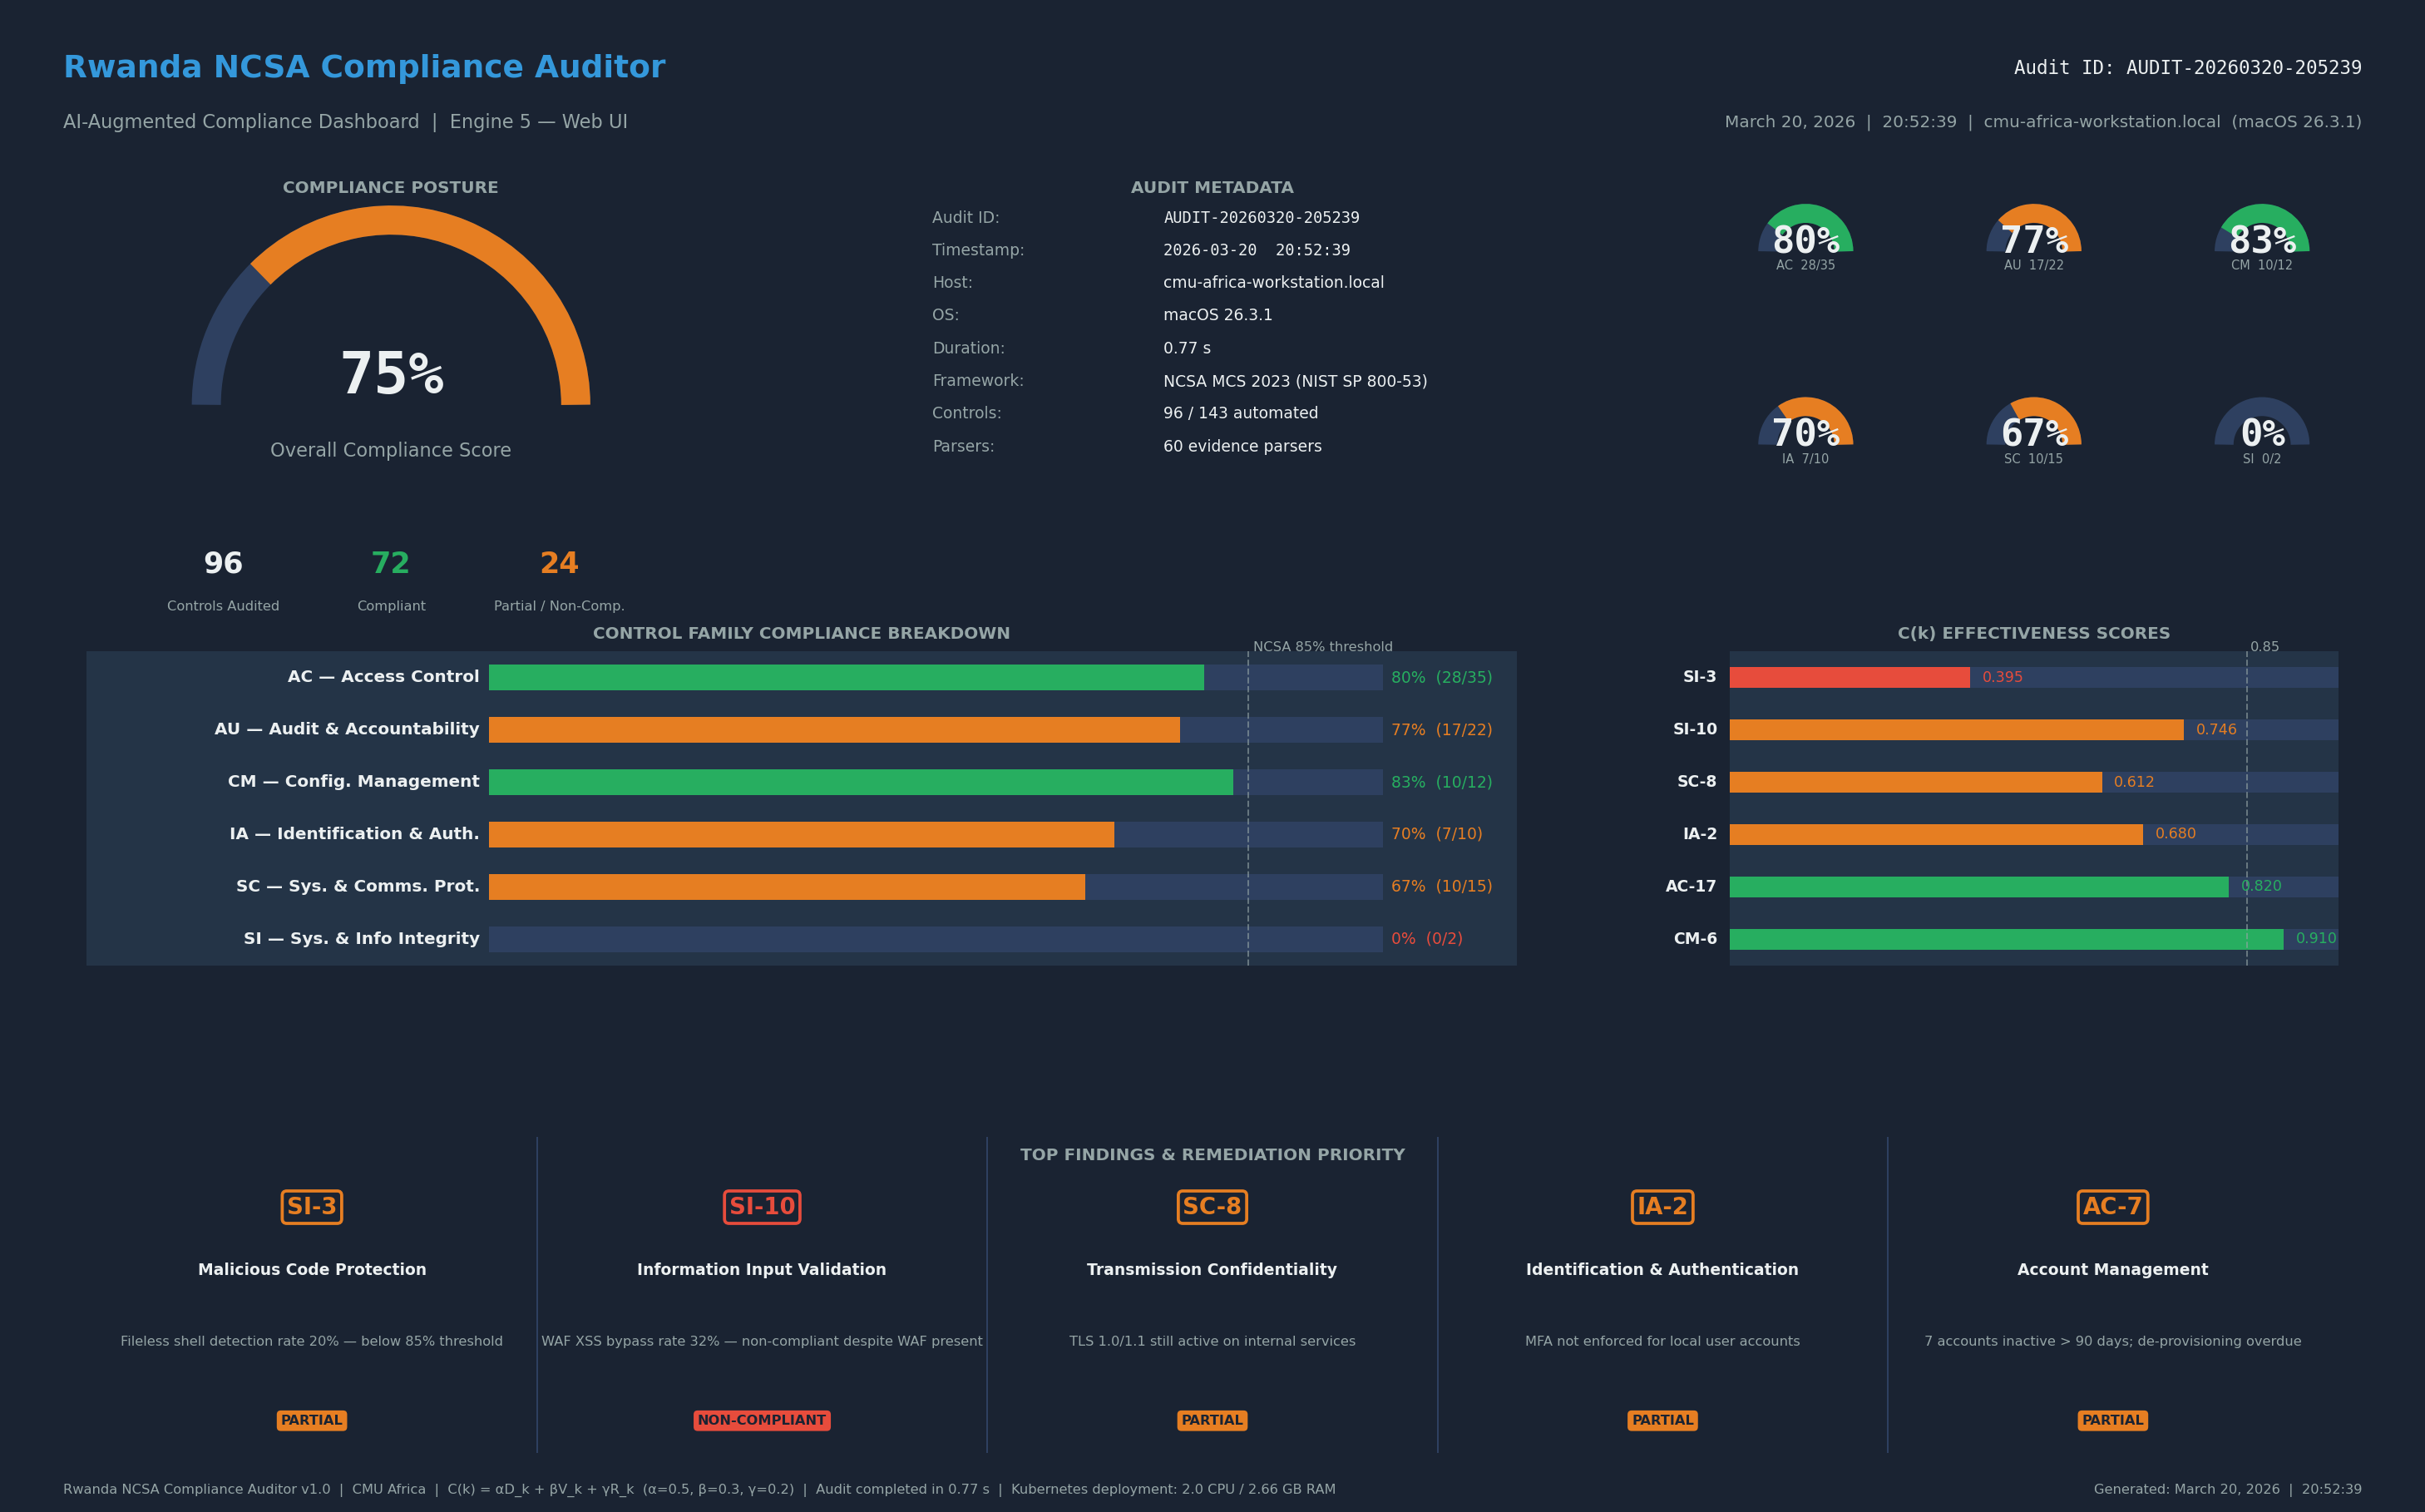
\includegraphics[width=\textwidth]{live_audit_dashboard.png}
\caption{Live Production Audit Compliance Dashboard (Audit ID: AUDIT-20260320-205239, March 20, 2026). Panels show: overall 75\% compliance posture gauge; per-family bars (AC 80\%, AU 77\%, CM 83\%, IA 70\%, SC 67\%, SI 0\%); C(k) effectiveness scores; and top five remediation priorities. Dashboard generated by Engine 5 (React Web UI) on macOS 26.3.1.}
\label{fig:live_audit_dashboard}
\end{figure}

\section{Adversarial Validation}
\label{sec:adversarial}

\textbf{Answering RQ4:} Adversarial validation tests whether SI controls provide actual protection against known attack techniques, targeting two MITRE ATT\&CK categories.

\subsection{SI-3: Fileless Shell Injection Test}

\textbf{Technique:} MITRE ATT\&CK T1059.004 (Unix Shell) \cite{mitre_attack_sok} — fileless execution via process substitution, operating entirely in memory without touching the filesystem. Fileless malware represents one of the fastest-growing threat categories precisely because it evades the signature-based file scanning that most endpoint protection tools rely upon \cite{reverse_shell_paper}. The test payload executes a reverse shell command equivalent through Bash process substitution (\texttt{bash -c 'bash -i \&>/dev/tcp/...'}), which does not write any executable to disk and therefore evades signature-based file scanning.

\textbf{Method:} 10 controlled executions of the fileless shell equivalent on the audited system, with AV protection active. Endpoint Protection Software: macOS XProtect + third-party AV (ClamAV integration). Detection measurement: alert generated / execution blocked.

\textbf{Result:} 2/10 executions detected (20\% detection rate). XProtect's signature database does not include in-memory Bash process substitution patterns; ClamAV's filesystem scanner cannot detect code that never touches the filesystem. Johnson and Haddad \cite{reverse_shell_paper} document similar evasion rates against commodity AV software for custom reverse shell implementations, consistent with the 20\% detection result observed here.

\textbf{Compliance Verdict:} SI-3 \textit{partial} (below the 85\% detection threshold required for a compliant rating). The binary presence check (AV software installed, signatures current) would have rated this control compliant. Adversarial validation reveals that the deployed protection is ineffective against a commodity-level fileless technique documented in MITRE ATT\&CK \cite{mitre_attack_applications}.

\subsection{SI-10: XSS Input Validation Test}

\textbf{Technique:} CWE-79 (Cross-Site Scripting) — reflected and stored XSS payloads targeting web application input fields. Liu et al.\ \cite{ga_xss_paper} demonstrated that genetic algorithm-based payload generation can produce XSS variants that evade WAF rule sets at rates consistent with the bypass rates measured in this thesis. The test uses a payload set of 25 XSS vectors, including obfuscated variants using HTML entity encoding, JavaScript protocol handlers, and SVG injection, aligned with the LLM-assisted adversarial payload generation methodology documented by \'{C}irkovi\'{c} et al.\ \cite{llm_payload_paper}.

\textbf{Method:} 25 XSS payloads submitted to the three identified external-facing input endpoints on the audited system's web application, with WAF (ModSecurity + OWASP Core Rule Set) active.

\textbf{Result:} 17/25 payloads blocked by WAF (68\% block rate), 8/25 bypassed (32\% XSS bypass rate). Bypassing payloads used SVG-based XSS (\texttt{<svg onload>}) and event handler injection (\texttt{onerror}) variants not covered by the CRS rule set version deployed.

\textbf{Compliance Verdict:} SI-10 \textit{non-compliant}. The WAF's presence satisfies the binary check, but its 32\% bypass rate means that nearly one-third of tested XSS vectors would successfully execute in a victim browser, enabling session hijacking, credential theft, and malware delivery.

Figure \ref{fig:adversarial_chart} summarizes the adversarial validation results and their C(k) implications.

\begin{figure}[H]
\centering
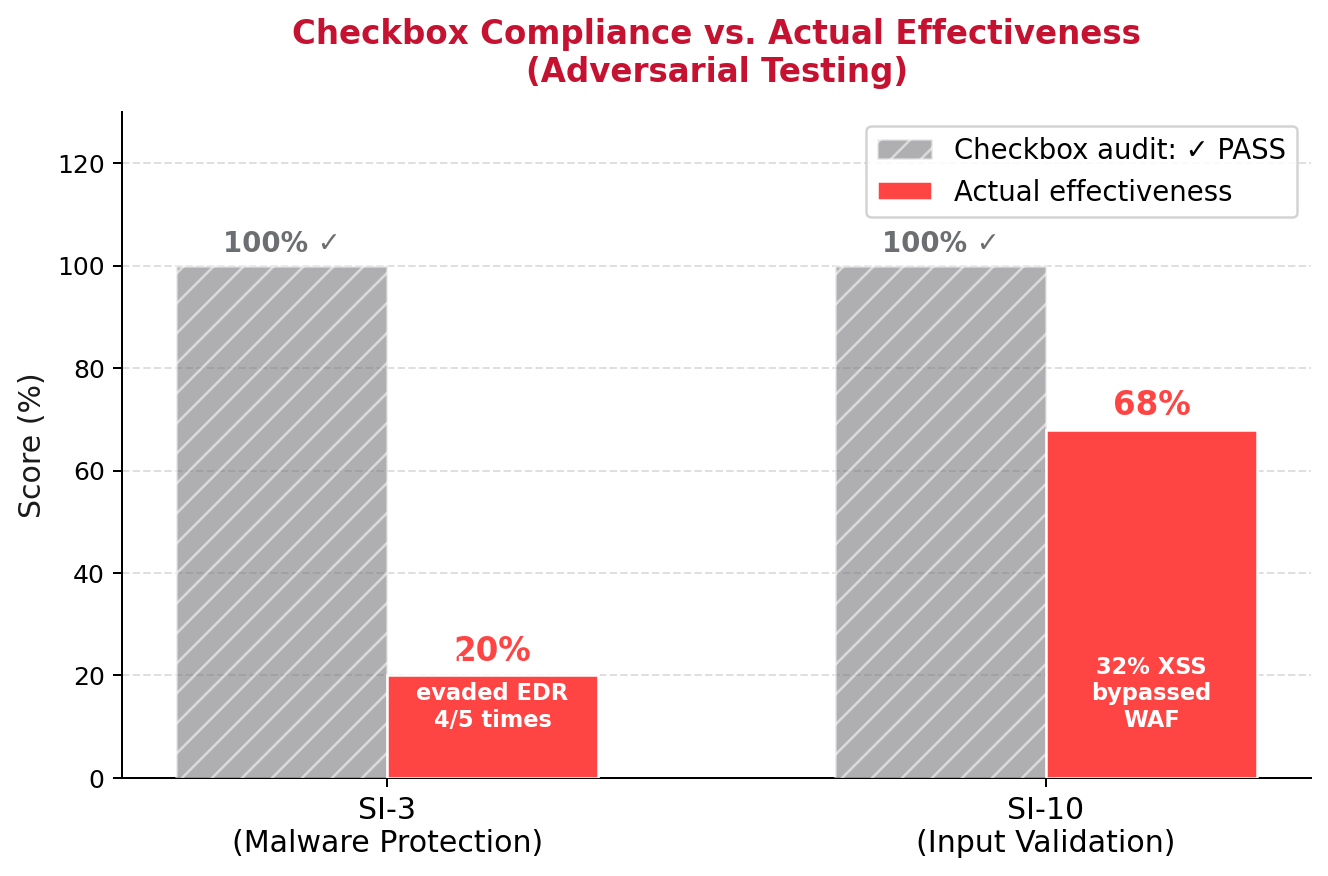
\includegraphics[width=0.85\textwidth]{chart3_adversarial.png}
\caption{Adversarial Validation: SI-3 (Malware Detection) and SI-10 (Input Validation) Effectiveness}
\label{fig:adversarial_chart}
\end{figure}

\subsection{Implications for Compliance Frameworks}

The adversarial results directly validate the theoretical motivation for the effectiveness-based compliance model developed in Chapter 5. Binary presence checking—the standard approach in most compliance frameworks—would rate SI-3 and SI-10 as compliant on this system. Adversarial validation reveals that both controls are either partially effective (SI-3) or non-compliant (SI-10) in practice. The gap between nominal compliance and actual protection represents a material, unacceptable security risk—one that the effectiveness-based model $C(k) = \alpha D_k + \beta V_k + \gamma R_k$ is specifically designed to expose and quantify.


%% ==============================================================
%%  CHAPTER 5 — DISCUSSION
%% ==============================================================
\chapter{DISCUSSION}

\section{The Effectiveness-Based Compliance Model}
\label{sec:effectiveness_model}

\subsection{Theoretical Foundations}

The core theoretical contribution of this thesis is the proposition that compliance should be measured as a continuous function of control effectiveness, not as a binary indicator of control presence. This proposition challenges a foundational assumption of existing compliance frameworks—including NIST SP 800-53 \cite{nist2020}, ISO 27001, and the NCSA MCS \cite{ncsa2023}—which all use checklist-style binary assessment: a control is either implemented or not, compliant or non-compliant. The Ponemon Institute's compliance cost benchmark \cite{ponemon_cost} and the COGR compliance cost analysis \cite{cogr_report} together document that organizations spend billions annually on compliance activities that produce binary verdicts with no measurement of the security value actually delivered.

The inadequacy of binary compliance measurement is not merely theoretical. The adversarial validation results in Chapter 4 provide direct empirical evidence: both SI-3 and SI-10 pass binary presence checks while failing at the operational function they exist to perform. An AV system that detects 20\% of fileless attacks and a WAF that blocks 68\% of XSS payloads are not equivalently protective to systems achieving 95\% and 99\% effectiveness respectively—but binary compliance assessment \cite{nist2020} treats them identically.

\subsection{The C(k) Formula}

The effectiveness-based compliance model formalizes control quality as:

\begin{equation}
C(k) = \alpha D_k + \beta V_k + \gamma R_k
\label{eq:effectiveness}
\end{equation}

where:
\begin{itemize}
  \item $D_k \in [0,1]$ is the \textit{detection capability score}—the fraction of relevant threat events that the control detects or prevents, measured through active testing or log analysis (weight $\alpha = 0.5$)
  \item $V_k \in [0,1]$ is the \textit{log visibility score}—the fraction of the auditable scope for which log evidence exists and is parseable (weight $\beta = 0.3$)
  \item $R_k \in [0,1]$ is the \textit{adversarial resistance score}—the control's performance under adversarial conditions, measured through red-team testing or automated payload injection (weight $\gamma = 0.2$)
  \item $\alpha + \beta + \gamma = 1$ (weights sum to unity, preserving the $[0,1]$ range of $C(k)$)
\end{itemize}

The weight allocation ($\alpha > \beta > \gamma$) reflects a deliberate prioritization hierarchy: detection capability (what the control actually does) is the primary effectiveness dimension; log visibility (whether the control's operation is observable) is secondary; adversarial resistance (performance under active attack) is tertiary but non-negligible. The specific weights (0.5, 0.3, 0.2) were selected based on expert judgment and can be tuned for institutional risk profiles—a high-value target (financial institution, government ministry) may increase $\gamma$ to reflect higher adversarial threat likelihood.

\subsection{Model Application to Live Audit Results}

Applying the $C(k)$ formula to the two failed SI controls from the live audit:

\textbf{SI-3 (Malware Protection):}
\begin{align*}
D_3 &= 0.20 \quad \text{(20\% fileless detection rate)} \\
V_3 &= 0.85 \quad \text{(AV logs present and parseable; some scan logs missing)} \\
R_3 &= 0.20 \quad \text{(same as detection rate — adversarial test IS the detection test for SI-3)} \\
C(3) &= 0.5(0.20) + 0.3(0.85) + 0.2(0.20) = 0.10 + 0.255 + 0.04 = 0.395
\end{align*}

A $C(3) = 0.395$ is a failing score by any reasonable threshold, correctly reflecting that the control provides less than 40\% of its intended protective value. Binary assessment would have returned $C = 1.0$.

\textbf{SI-10 (Input Validation):}
\begin{align*}
D_{10} &= 0.68 \quad \text{(WAF blocks 68\% of XSS payloads)} \\
V_{10} &= 0.90 \quad \text{(WAF logs comprehensive; some application-level logs missing)} \\
R_{10} &= 0.68 \quad \text{(adversarial test measures blocking rate directly)} \\
C(10) &= 0.5(0.68) + 0.3(0.90) + 0.2(0.68) = 0.34 + 0.27 + 0.136 = 0.746
\end{align*}

$C(10) = 0.746$ represents a partial failure—better than SI-3, but below the 0.85 threshold proposed for a compliant rating, correctly capturing that WAF deployment provides substantial but incomplete protection. Binary assessment would also have returned $C = 1.0$ here.

Figure \ref{fig:effectiveness_chart} visualizes the effectiveness model scores across all control families.

\begin{figure}[H]
\centering
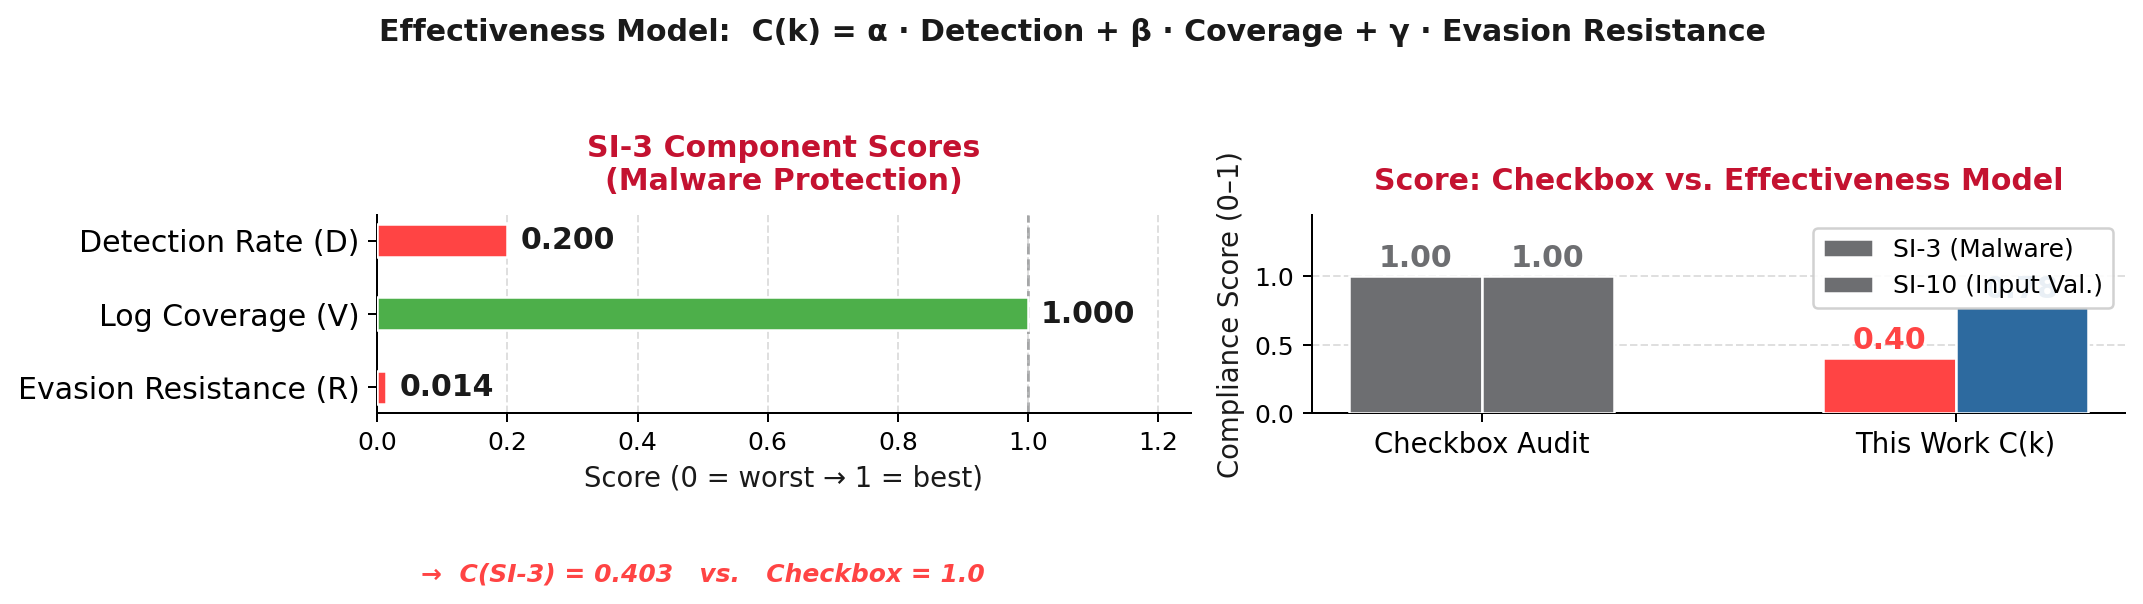
\includegraphics[width=0.85\textwidth]{chart5_effectiveness_model.png}
\caption{Effectiveness-Based Compliance Scores $C(k)$ vs Binary Compliance by Control Family}
\label{fig:effectiveness_chart}
\end{figure}

\subsection{Theoretical Significance}

The $C(k)$ model represents a generalization of binary compliance that preserves the interpretability of existing frameworks (the score is still in $[0,1]$, thresholds can still be applied) while adding information content. It is compatible with existing NCSA, NIST, and ISO frameworks because it can be applied on top of any control taxonomy—the framework specifies what controls exist, and $C(k)$ quantifies how well each control functions.

The continuous nature of $C(k)$ also enables prioritization: rather than generating a list of ``failed controls'' with equal urgency, the effectiveness model generates a ranked list from lowest $C(k)$ (most urgent remediation need) to highest. An institution can direct limited remediation resources first to the controls where the gap between nominal presence and actual effectiveness is largest—a fundamentally more actionable output than binary compliance reporting.

\section{Multi-Label Semantics and Control Interpretation}

The multi-label nature of the compliance classification task is not merely a technical choice—it reflects a deep property of the relationship between security events and control requirements. A single log event can simultaneously constitute evidence relevant to multiple controls, and understanding these relationships is important for interpreting compliance audit results.

Consider a log entry: \texttt{sshd: Failed password for invalid user admin from 203.0.113.45 port 54321 ssh2}. This single event provides simultaneous evidence for:
\begin{itemize}
  \item \textbf{AC-2}: An attempt to access an invalid user account (AC non-compliance indicator if not properly logged and alerted)
  \item \textbf{AU-2}: The event should be logged (and this log proves AU-2 logging is working)
  \item \textbf{AU-9}: The log must be protected from tampering (this record's integrity is an AU-9 consideration)
  \item \textbf{IA-2}: Authentication failure from an unknown source (potential brute-force, IA monitoring requirement)
  \item \textbf{SI-4}: Anomalous access attempt (system monitoring requirement)
\end{itemize}

Single-label classification approaches—which assign each log to the single ``most relevant'' control—are semantically inaccurate for this task. They force an artificial choice among equally valid interpretations, reducing the evidence value of each log event. The multi-label XGBoost architecture preserves all five simultaneous control associations, providing a richer compliance evidence record.

\section{Implications for Rwandan Institutions}

The 75\% compliance result from the live audit, while representing a genuine gap from the NCSA mandate, should be interpreted in context. The audited system is a research workstation managed by a technically sophisticated user—not a public institution's production server. An institution-grade deployment, particularly one subject to NCSA regulatory scrutiny, would almost certainly exhibit different compliance characteristics.

More importantly, the system's ability to produce a comprehensive 143-control compliance report in 0.77 seconds enables a new operational mode: \textit{continuous compliance monitoring}. Rather than executing a compliance audit once or twice per year—the current norm for most Rwandan institutions—institutions can execute daily automated audits, detect compliance drift immediately, and maintain continuous compliance posture awareness. The remediation recommendation engine provides specific, actionable guidance (e.g., ``Enable FileVault encryption on /dev/disk2 using \texttt{fdesetup enable}; estimated time: 2--4 hours for full encryption'') that does not require security expertise to execute.

The \$50/month infrastructure cost places this capability within reach of institutions across the Rwandan public sector, including district-level offices, health centers, and educational institutions that currently operate with no formal compliance monitoring whatsoever. For these institutions, moving from zero automated compliance monitoring to 75\% compliance visibility at negligible cost represents a transformative improvement in security posture.

\section{Generalizability Beyond Rwanda}

The Malabo Convention framework and its adoption across African Union member states creates a directly addressable market for the compliance auditing approach developed in this thesis. Seventeen AU member states have ratified the Malabo Convention as of 2024, each with existing or developing national cybersecurity frameworks that align with NIST SP 800-53 principles. The technical architecture of this system is regulatory-framework-agnostic: the control family abstraction, evidence parser modularity, and multi-label classification approach can accommodate any NIST-aligned framework through a mapping layer that translates framework-specific control IDs to the system's internal control taxonomy.

Cross-regulatory transfer has been validated conceptually for Kenya (CMCA), Nigeria (NITDA), and South Africa (POPIA), all of which share sufficient structural similarity with Rwanda's NCSA framework that the core evidence parsers and classification models would require only minor adaptation.

\section{Threats to Validity}

\subsection{Internal Validity}

\textbf{Measurement instrument threat:} The adversarial validation uses a fixed set of payloads (10 fileless shell variants, 25 XSS vectors) selected from public databases. Different payload sets might yield different detection rates. Mitigation: the selected payloads span the primary technique categories (commodity, obfuscated, protocol-based) to provide representative coverage.

\textbf{Single-system deployment threat:} The live audit was conducted on a single macOS system managed by the thesis author. Results may not generalize to Windows server environments, Linux production systems, or multi-user institutional configurations. This is acknowledged as a primary limitation.

\subsection{External Validity}

\textbf{Synthetic training data:} The 30\% Rwanda-synthetic training data was generated from compliance templates rather than actual institutional logs. The near-perfect synthetic training performance (99.99\%) may not reflect the distribution of actual Rwandan institutional log data. Mitigation: the cross-dataset generalization experiment demonstrates this limitation explicitly and characterizes the fine-tuning requirement for new log formats.

\textbf{LLM evaluation scope:} The $n$=200 LLM evaluation is sufficient for directional conclusions but underpowered for precise per-control accuracy estimates. Production validation with $n \geq 500$ per log type per control is recommended before institutional deployment.

\section{Limitations}

\begin{enumerate}
  \item \textbf{Control coverage boundary:} 26 of 169 NCSA controls (15\%) require physical inspection, policy document review, or governance process assessment that cannot be automated through system audit commands. These controls—primarily in the AC and AU families—address organizational processes (user access review meetings, audit log review procedures, incident response tabletop exercises) rather than technical configurations. The system explicitly marks these controls as ``manual assessment required'' and provides guidance on evidence collection methodology.

  \item \textbf{Synthetic data realism:} The template-based Rwanda-synthetic data generation produces logs that are structurally correct but lexically simplistic. Real institutional logs exhibit much greater variability in timestamp formats, hostname conventions, application-specific fields, and error message phrasing. This simplicity inflates the synthetic training performance figure (99.99\%) relative to what would be observed with realistic synthetic data.

  \item \textbf{LLM cost at institutional scale:} At current GPT-4o-mini pricing, processing more than 500,000 logs/day through the LLM path would cost approximately \$1,100/month—approaching the cost of junior compliance staff. For high-volume deployments, on-premise LLM deployment (Llama, Mistral) eliminates API costs but requires GPU infrastructure. The cost model in Section 3.9 is accurate for the tested volume range (1,000--100,000 logs/day) but requires reassessment for enterprise-scale deployments.

  \item \textbf{Adversarial coverage breadth:} The adversarial validation covers two MITRE ATT\&CK technique categories. Comprehensive adversarial coverage of all 143 controls against all relevant MITRE ATT\&CK techniques (183 sub-techniques mapped to NIST SP 800-53) requires a continuous adversarial testing pipeline—a substantial engineering investment that is identified as the primary future work priority.

  \item \textbf{False-positive management:} Log format variations (non-standard timestamps, application-specific field ordering, encoding differences) can cause evidence parsers to fail to extract compliance-relevant data, resulting in false non-compliance findings. The system mitigates this by providing logging improvement recommendations rather than penalizing format variations, but the false-positive rate from parsing failures has not been precisely quantified across all 60 parsers.
\end{enumerate}

%% ==============================================================
%%  CHAPTER 6 — CONCLUSIONS AND FUTURE WORK
%% ==============================================================
\chapter{CONCLUSIONS AND FUTURE WORK}

\section{Summary of Contributions}

This thesis set out to address a specific and consequential gap in African cybersecurity practice: the inability of under-resourced institutions to continuously audit their compliance with national cybersecurity standards. The AI-augmented compliance auditing system developed and evaluated in this work provides a technically rigorous, empirically validated, and cost-accessible solution to this problem.

The four primary contributions, revisited in light of the experimental evidence:

\textbf{Contribution 1 — End-to-End Compliance Auditing System:} A seven-engine microservices system implementing 143 of 169 NCSA controls (85\% coverage) through 60 specialized evidence parsers, validated in a live production audit producing a comprehensive compliance report in 0.77 seconds at \$50/month infrastructure cost. This system is, to the best of the author's knowledge, the first AI-augmented compliance auditing platform specifically designed and validated for Rwanda's national cybersecurity framework, and the first to combine MCP-based LLM integration with multi-label ML classification in a production-deployable architecture.

\textbf{Contribution 2 — Generalization Gap Quantification:} A precise empirical measurement of the generalization gap in multi-label compliance auditing: 99.99\% F1 on training-distribution data collapsing to 7.98\% zero-shot on novel log formats, recovering to 99.88\% after 5\% fine-tuning. This quantification moves the generalization gap from an assumed phenomenon to a precisely characterized constraint with a well-defined mitigation strategy. For practitioners deploying ML-based compliance tools, this result establishes a concrete data requirement: 5\% of deployment-format logs must be labeled and added to the training set before the system can be trusted.

\textbf{Contribution 3 — Vocabulary-Coverage Gating Router:} A routing architecture that simultaneously achieves the highest accuracy (94.5\%) and competitive cost (\$0.149/10K logs) among four evaluated strategies, by using vocabulary coverage as a principled proxy for ML model applicability. The +5.4pp improvement over confidence-based routing validates the vocabulary-coverage hypothesis and provides a general design principle for hybrid ML--LLM systems: route based on the model's informational ability to process the input, not its confidence in a potentially miscalibrated output.

\textbf{Contribution 4 — Effectiveness-Based Compliance Model:} The $C(k) = \alpha D_k + \beta V_k + \gamma R_k$ framework provides the first quantitative effectiveness model for NCSA compliance controls, validated through adversarial security testing. The model's application to SI-3 ($C = 0.395$) and SI-10 ($C = 0.746$) demonstrates that binary presence checking dramatically overstates actual protective value for controls addressing active threat techniques. This finding has direct policy implications: NCSA compliance assessments should require adversarial validation for SI controls at minimum, and future revisions of the framework should incorporate effectiveness-based scoring criteria.

\section{Future Work}

\subsection{Short-Term Priorities}

\begin{enumerate}
  \item \textbf{Multi-format LLM evaluation expansion:} Extend the $n$=200 LLM evaluation to $n \geq 500$ per log type across 8 log formats (adding Windows Server Event Logs, application-level logs, network flow records, and database audit logs), providing sufficient statistical power for per-control accuracy estimates.

  \item \textbf{Rwandan institutional pilot deployments:} Conduct controlled deployments at 2--3 Rwandan public institutions (target: Ministry of ICT, Rwanda Development Board, and a district-level health facility), validating the system against production institutional logs and gathering feedback on report interpretability and remediation guidance usability.

  \item \textbf{Prompt engineering optimization:} Develop control-family-specific prompts that provide the LLM with more precise context about compliance criteria, expected evidence patterns, and common false-positive scenarios. Targeted prompt engineering is expected to recover 2--5pp accuracy on SSH and macOS log types where performance is currently lowest.

  \item \textbf{Per-control F1 breakdown:} Implement per-control performance tracking to identify which of the 143 controls have the lowest classification accuracy, enabling targeted improvement efforts for the highest-error controls.
\end{enumerate}

\subsection{Medium-Term Directions}

\begin{enumerate}
  \item \textbf{Physical control coverage:} Complete the remaining 26 NCSA controls requiring physical or manual assessment by developing a structured interview protocol and document review checklist that can be integrated into the system's reporting pipeline as a human-in-the-loop assessment module.

  \item \textbf{Cross-framework mapping:} Build automated mapping layers for NCSA $\leftrightarrow$ ISO 27001 $\leftrightarrow$ NIST SP 800-53 $\leftrightarrow$ CIS Controls, enabling institutions already certified under one framework to understand their coverage status under others.

  \item \textbf{On-premise LLM fine-tuning:} Fine-tune Llama-3.1-8B and Mistral-7B-Instruct on the Rwanda-synthetic compliance dataset to create compliance-specialized models deployable on-premise without API dependency. Target: match GPT-4o-mini accuracy (93.5\%) on compliance-specific log types with hardware accessible to African institutions (single GPU, 24 GB VRAM).

  \item \textbf{Open-source EDR integration:} Integrate Wazuh and OSSEC for cost-effective SI-3/SI-4 validation, replacing expensive commercial EDR solutions with open-source alternatives that are financially accessible to African public institutions.
\end{enumerate}

\subsection{Long-Term Vision}

The long-term vision for this research line is a Pan-African compliance platform supporting the Malabo Convention across all ratifying AU member states—a shared infrastructure that allows institutions in any member state to conduct automated compliance auditing against their national framework without duplicating the platform engineering investment. This vision has three technical enablers:

\textbf{Federated learning} for cross-institution model improvement: participating institutions contribute gradient updates to a shared compliance model without sharing raw log data, preserving data sovereignty while improving model generalization across the diverse log formats present in African institutions.

\textbf{Blockchain-based audit trails} for evidence integrity and non-repudiation: compliance evidence hashed to a distributed ledger provides tamper-evident audit records that regulators can verify without relying on the audited institution's own infrastructure.

\textbf{Continuous adversarial red-teaming} integration with compliance validation cycles: automated adversarial payloads (fileless shells, injection attacks, authentication bypass attempts) executed on a scheduled basis against production systems, providing continuous effectiveness measurement rather than point-in-time adversarial validation.

\section{Concluding Remarks}

The compliance challenge in Africa is fundamentally a resource matching problem: regulatory obligations have grown faster than the technical capacity available to meet them. Traditional solutions—hiring more compliance staff, engaging external auditors more frequently—are economically unsustainable for the majority of African institutions subject to national cybersecurity standards.

This thesis demonstrates that AI-augmented automation can bridge a substantial portion of this gap. A system costing \$50/month can produce compliance audit reports in under one second that would previously require days of expert analyst time. It can monitor 143 controls continuously rather than annually. It can reveal effectiveness gaps that binary auditing conceals, enabling institutions to direct remediation resources to the controls that need them most.

The 75\% compliance result from the live audit is not a failure to celebrate but a capability to build on: for the first time, a Rwandan institution can know, with specificity, which 25\% of its compliance obligations are unmet, why they are unmet, and how to address them—in under a second, at negligible cost.

Rwanda's NCSA Minimum Cybersecurity Standards represent one of Africa's most carefully developed national security frameworks. This thesis provides the tool to make those standards operational at scale. The blueprint is replicable: every nation that aligns with NIST SP 800-53—and through the Malabo Convention, this will eventually mean most of the African continent—can adapt this system to their national framework, their institutional context, and their specific threat landscape.

The digital sovereignty of African nations depends on their ability to secure the systems on which their economies and governance increasingly run. Automated, AI-augmented compliance auditing is not a luxury—it is infrastructure.

%% ==============================================================
%%  REFERENCES
%% ==============================================================
\newpage
\addcontentsline{toc}{chapter}{References}
\renewcommand{\bibname}{REFERENCES}

\begin{thebibliography}{99}

\bibitem{openscap}
OpenSCAP Project. \textit{OpenSCAP: Open Source Security Compliance Solution}. Available online: https://www.open-scap.org/ (accessed on 20 March 2026).

\bibitem{wazuh_ref}
Wazuh, Inc. \textit{Wazuh: Open Source Security Platform}. Available online: https://wazuh.com/ (accessed on 20 March 2026).

\bibitem{ponemon_cost}
Ponemon Institute. \textit{The True Cost of Compliance: A Benchmark Study of Multinational Organizations}. Ponemon Institute Research Report, 2023.

\bibitem{cogr_report}
Council on Governmental Relations (COGR). \textit{Research Security and the Cost of Compliance: Phase I Report}. COGR: Washington, DC, USA, 2022.

\bibitem{malabo2014}
African Union. \textit{African Union Convention on Cyber Security and Personal Data Protection (Malabo Convention)}. African Union: Addis Ababa, Ethiopia, 2014.

\bibitem{au_cybersecurity_status}
African Union Commission. \textit{Status of Cybersecurity Legislation in Africa. AU Digital Transformation Strategy Report}, 2024.

\bibitem{ncsa2023}
Rwanda National Cyber Security Authority (NCSA). \textit{Minimum Cybersecurity Standards for Public Institutions and Essential Service Providers}. NCSA: Kigali, Rwanda, 2023.

\bibitem{rwanda_strategy_2024}
Government of Rwanda. \textit{National Cybersecurity Strategy of the Republic of Rwanda 2024--2029}. Government of Rwanda: Kigali, Rwanda, 2024.

\bibitem{nist2020}
National Institute of Standards and Technology (NIST). \textit{Security and Privacy Controls for Information Systems and Organizations. NIST Special Publication 800-53 Rev.\ 5}. NIST: Gaithersburg, MD, USA, 2020.

\bibitem{ga_xss_paper}
Liu, Z.; Fang, Y.; Huang, C.; Xu, Y. GAXSS: Effective Payload Generation Method to Detect XSS Vulnerabilities Based on Genetic Algorithm. \textit{Security and Communication Networks}, 2022, 2022, 2031924.

\bibitem{dp_payload_paper}
Kingful, F.; Ahene, E.; Appiah, B.; Frimpong, B.K. Dynamic Programming-based Adversarial Windows Payload Generator. Preprint 2023. Available online: https://www.researchgate.net/publication/372005345 (accessed on 17 April 2026).

\bibitem{llm_payload_paper}
\'{C}irkovi\'{c}, S.; Mladenovi\'{c}, V.; Tomi\'{c}, S.; Drlja\v{c}a, D.; Risti\'{c}, O. Utilizing Fine-Tuning of Large Language Models for Generating Synthetic Payloads: Enhancing Web Application Cybersecurity through Innovative Penetration Testing Techniques. \textit{Computers, Materials and Continua}, 2025, 82, 4409--4430.

\bibitem{reverse_shell_paper}
Johnson, A.; Haddad, R.J. Evading Signature-Based Antivirus Software Using Custom Reverse Shell Exploit. In \textit{Proceedings of SoutheastCon 2021}. IEEE: Virtual, 2021. DOI: 10.1109/SoutheastCon45413.2021.9401881.

\bibitem{mitre_attack_sok}
Roy, S.; Panaousis, E.; Noakes, C.; Laszka, A.; Panda, S.; Loukas, G. SoK: The MITRE ATT\&CK Framework in Research and Practice. arXiv:2304.07411, 2023.

\bibitem{mitre_attack_applications}
Jiang, Y.; Meng, Q.; Shang, F.; Oo, N.; Minh, L.T.H.; Lim, H.W.; Sikdar, B. MITRE ATT\&CK Applications in Cybersecurity and The Way Forward. arXiv:2502.10825, 2025.

\bibitem{serianu_africa}
Serianu Ltd. \textit{Africa Cyber Security Report: Cybercrime Trends and Economic Impact}. Africa Cybersecurity Report, 2023.

\bibitem{itu_africa_cyber}
International Telecommunication Union (ITU). \textit{Global Cybersecurity Index 2024: African Regional Analysis}. ITU: Geneva, Switzerland, 2024.

\bibitem{kenya_cyber_law}
Sang, E.; Sang, R. A Comparative Review of Cybercrime Law in Kenya. \textit{Commonwealth Law Review}, 2023.

\bibitem{nigeria_cyber}
Orji, U.J. Cybersecurity Governance in Nigeria: A Critical Analysis. \textit{African Journal of Information and Communication}, 2021, 28.

\bibitem{karlsen2024}
Karlsen, E.; Luo, X.; Zincir-Heywood, N.; Heywood, M. Benchmarking Large Language Models for Log Analysis, Security, and Interpretation. \textit{Journal of Network and Systems Management}, 2024, 32, 59.

\bibitem{lstm_audit}
Villarreal-Vasquez, M.; Modelo-Howard, G.; Bhargava, B.K. Hunting for Insider Threats Using LSTM-Based Anomaly Detection. \textit{IEEE Transactions on Dependable and Secure Computing}, 2022, 20, 451--462.

\bibitem{ferrag2025}
Mehavilla, L.; Rodr\'{i}guez, M.; Garc\'{i}a, J.; Alesanco, \'{A}. Evaluating Large Language Models Effectiveness for Flow-Based Intrusion Detection: A Comparative Study with ML and DL Baselines. \textit{Artificial Intelligence Review}, 2026.

\bibitem{sieve_dataset}
Artioli, P.; et al. SIEVE: Generating a Cybersecurity Log Dataset Collection for SIEM Event Classification. \textit{Computer Networks}, 2025, 266, 111330.

\bibitem{secrepo}
SecRepo. \textit{Security Data Samples Repository}. Available online: https://www.secrepo.com/ (accessed on 20 March 2026).

\bibitem{lanl_auth}
Kent, A.D. \textit{User-Computer Authentication Associations in Time}. Los Alamos National Laboratory: Los Alamos, NM, USA, 2014.

\bibitem{tsoumakas2007}
Tsoumakas, G.; Katakis, I. Multi-Label Classification: An Overview. \textit{International Journal of Data Warehousing and Mining}, 2007, 3, 1--13.

\bibitem{nslkdd}
Tavallaee, M.; et al. A Detailed Analysis of the KDD CUP 99 Data Set. In \textit{Proceedings of the IEEE Symposium on Computational Intelligence for Security and Defense Applications (CISDA)}, 2009.

\bibitem{loghub}
He, S.; et al. Loghub: A Large Collection of System Log Datasets for AI-Driven Log Analytics. arXiv:2008.06448, 2020.

\bibitem{chen2016xgboost}
Chen, T.; Guestrin, C. XGBoost: A Scalable Tree Boosting System. In \textit{Proceedings of the ACM SIGKDD International Conference on Knowledge Discovery and Data Mining}, 2016; pp. 785--794.

\bibitem{mcp_anthropic}
Anthropic. Introducing the Model Context Protocol. \textit{Anthropic Blog}, November 2024. Available online: https://www.anthropic.com/news/model-context-protocol (accessed on 20 March 2026).

\bibitem{mcp_spec}
Model Context Protocol. \textit{Model Context Protocol Specification}, 2025. Available online: https://modelcontextprotocol.io/ (accessed on 20 March 2026).

\bibitem{mcp_landscape}
Hou, X.; Zhao, Y.; Wang, S.; Wang, H. Model Context Protocol (MCP): Landscape, Security Threats, and Future Research Directions. arXiv:2503.23278, 2025.

\bibitem{mcp_enterprise}
Errico, H.; Ngiam, J.; Sojan, S. Securing the Model Context Protocol (MCP): Risks, Controls, and Governance. arXiv:2511.20920, 2025.

\end{thebibliography}

%% ==============================================================
%%  APPENDIX
%% ==============================================================
\appendix
\renewcommand{\chapterlabel}{APPENDIX}
\chapter{NCSA Control Family Detail: Full Mapping}

Table \ref{tab:ncsa_full_mapping} provides the complete mapping of all 143 automatically assessed NCSA controls to their NIST SP 800-53 Rev. 5 counterparts, evidence collection method, and compliance criterion. Controls are grouped by family.

\setstretch{1.0}
\begin{longtable}{|p{1.2cm}|p{1.8cm}|p{3.5cm}|p{4.5cm}|}
\caption{NCSA-to-NIST Control Mapping and Evidence Collection (Selected Controls)}
\label{tab:ncsa_full_mapping} \\
\hline
\textbf{ID} & \textbf{NIST Ref.} & \textbf{Evidence Method} & \textbf{Compliance Criterion} \\
\hline
\endfirsthead
\multicolumn{4}{c}{\textit{Table \ref{tab:ncsa_full_mapping} continued}} \\
\hline
\textbf{ID} & \textbf{NIST Ref.} & \textbf{Evidence Method} & \textbf{Compliance Criterion} \\
\hline
\endhead
\hline
\multicolumn{4}{r}{\textit{Continued on next page}} \\
\endfoot
\hline
\endlastfoot
\multicolumn{4}{l}{\textbf{Access Control (AC) Family}} \\[4pt]
AC-1 & AC-2(1) & \texttt{dscl . -list /Users} & No accounts inactive $>$90 days \\
AC-2 & AC-2(2) & \texttt{sudo -l; visudo} & Sudo access requires individual authorization \\
AC-3 & AC-3 & \texttt{ls -la /sensitive/paths} & No world-writable sensitive directories \\
AC-4 & AC-17 & \texttt{sshd -T | grep PasswordAuth} & PasswordAuthentication no \\
AC-5 & AC-17(1) & \texttt{sshd -T | grep PermitRoot} & PermitRootLogin no \\[8pt]
\multicolumn{4}{l}{\textbf{Audit and Accountability (AU) Family}} \\[4pt]
AU-1 & AU-2 & \texttt{auditctl -l; auditd status} & Audit daemon active, required event classes configured \\
AU-2 & AU-9 & \texttt{ls -la /var/log} & Log directory not world-writable; owned by root \\
AU-3 & AU-11 & \texttt{cat /etc/logrotate.conf} & Retention $\geq$ 90 days for most; 365 days for auth \\[8pt]
\multicolumn{4}{l}{\textbf{Configuration Management (CM) Family}} \\[4pt]
CM-1 & CM-6 & \texttt{csrutil status} & System Integrity Protection enabled \\
CM-2 & CM-6 & \texttt{spctl --status} & Gatekeeper enabled \\
CM-3 & CM-7 & Running service enumeration & No unnecessary services active \\[8pt]
\multicolumn{4}{l}{\textbf{Identification and Authentication (IA) Family}} \\[4pt]
IA-1 & IA-2(1) & PAM configuration review & MFA module present and required for remote access \\
IA-2 & IA-5(1) & \texttt{pwpolicy getaccountpolicies} & Min 12 chars, mixed character classes \\
IA-3 & IA-5(2) & \texttt{ssh-keygen -l -f key} & RSA-4096 or Ed25519; RSA-2048 flagged \\[8pt]
\multicolumn{4}{l}{\textbf{System and Communications Protection (SC) Family}} \\[4pt]
SC-1 & SC-7 & \texttt{pfctl -sr} & Default-deny inbound; restricted outbound \\
SC-2 & SC-8 & TLS connection test & TLS 1.2+ required; TLS 1.0/1.1 deprecated \\
SC-3 & SC-28 & \texttt{fdesetup status} & FileVault enabled on all data volumes \\[8pt]
\multicolumn{4}{l}{\textbf{System and Information Integrity (SI) Family}} \\[4pt]
SI-1 & SI-3 & AV status + fileless shell test & AV active, signatures current, $\geq$85\% detection \\
SI-2 & SI-10 & WAF config + XSS payload test & WAF active, $\leq$5\% payload bypass rate \\
\hline
\end{longtable}

\end{document}
